\documentclass[11pt]{article}
\usepackage{graphicx}
\usepackage{hyperref}
\usepackage{caption}
\usepackage{amsmath}
\usepackage{mathtools}
\usepackage{physics}
\newcommand{\numpy}{{\tt numpy}}    % tt font for numpy

\topmargin -.5in
\textheight 9in
\oddsidemargin -.25in
\evensidemargin -.25in
\textwidth 7in

\begin{document}

% ========== Edit your name here
\author{Hongqing Liu, hl85}
\title{CS 498: Assignment 2: Multi-view Geometry}
\date{February 23, 2023}
\maketitle

\medskip


\section*{Submission}
In this assignment you will code your own structure-from-motion and stereo matching algorithm to convert 2D observations to 3D structures. The starter code consists of 4 python files you will modify along with a folder of some images and saved data. Please put together a single PDF with your answers and figures for each problem, and submit it to Gradescope (Course Code: BBX6NE). If your code produces figures they should go in this pdf, along with a description of what you did to solve the problem. We recommend you to use the latex template files we provided. For code submission, make sure you upload the provided ``.py" files with your modifications. The graders will check both your PDF submission and your code submission if needed. 

\section*{Keypoint Matching} 
\paragraph{Question 1 (Putative Matches) [2 pts]:} Here you will be modifying ``correspondence.py". Your task is to select putative matches between detected SIFT keypoints found in two images. Detecting keypoints will be done for you by cv2. The matches should be selected based on the Euclidean distance between the pairwise descriptors. In your implementation, make sure to filter your keypoint matches using Lowe's ratio test (\href{https://stackoverflow.com/questions/51197091/how-does-the-lowes-ratio-test-work}{link}).  For this question, you should implement your solution without using third-party functions e.g., cv2 knnmatch, which can significantly trivialize the problem. Meanwhile, please avoid solutions using for-loop which slows down the calculations. \textbf{Hint}: To avoid using for-loop, check out \texttt{scipy.spatial.distance.cdist (X,Y,'sqeuclidean')}.

\textbf{Answer: } The result of matches is shown as follows, based on the result, when the ratio is small, the matches has better performance.
\begin{center}
    \small
    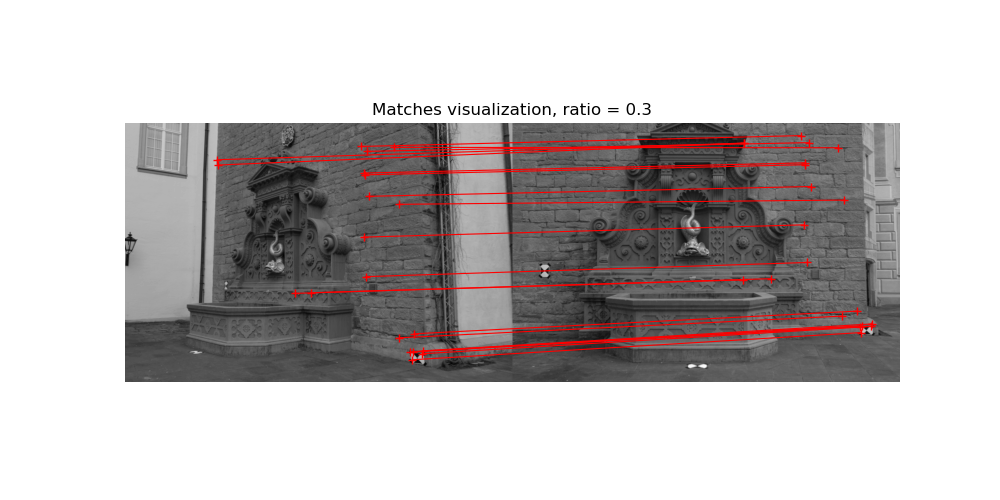
\includegraphics[width=0.3\linewidth]{fig/pic1ratio0.3.png}
    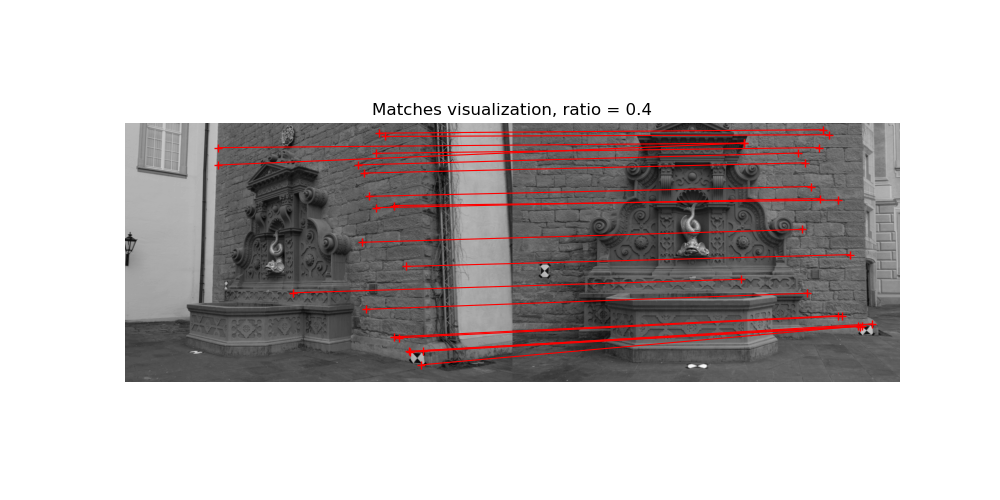
\includegraphics[width=0.3\linewidth]{fig/pic1ratio4.png}
    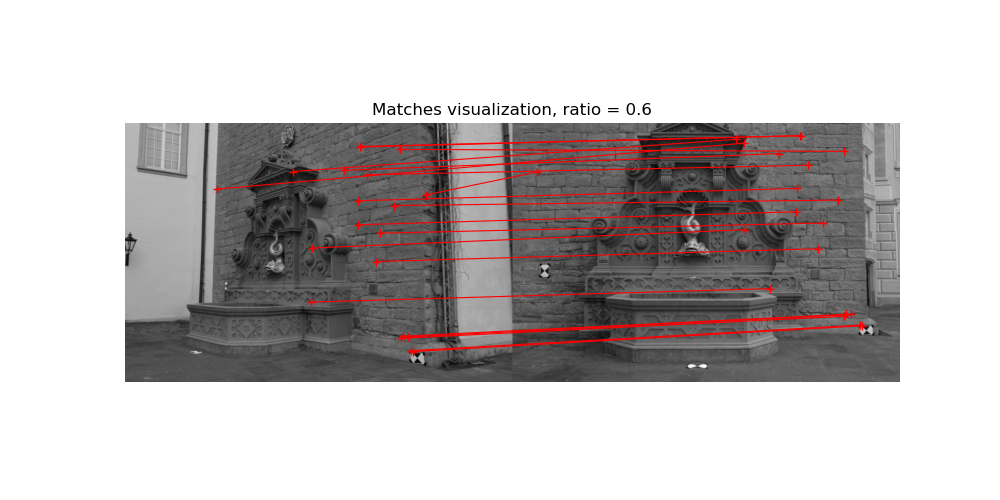
\includegraphics[width=0.3\linewidth]{fig/pic1ratio0.6.png}
\end{center}

\section*{Fundamental Matrix Estimation} 

\paragraph{Question 2 (Eight-point Estimation) [3 pts]:} Here you will be modifying ``fundamental.py". For this question, your task is to implement the unnormalized eight-point algorithm (covered in class lecture) and normalized eight-point algorithm (\href{https://en.wikipedia.org/wiki/Eight-point_algorithm#Normalized_algorithm}{link}) to find out the fundamental matrix between two cameras. We provide code to compute the quality of your matrices based on the average geometric distance, i.e. the distance between each projected keypoint from one image to its corresponding epipolar line in the other image. Please report this distance in your pdf.

\textbf{Amswer: } In this question, I use the following function to normalized the points. T is the transformation matrix to normalize points and $s$ is the scale factor while $t_x$, $t_y$ are centroid of the points.

\[T = 
\left[
\begin{array}{ccc}
    s & 0 & -st_x \\
    0 & s & -st_y \\
    0 & 0 & 1
\end{array}
\right]
\]

The normalized function, rank2 codes and denormalization part are shown as follows:

\begin{center}
    \small
    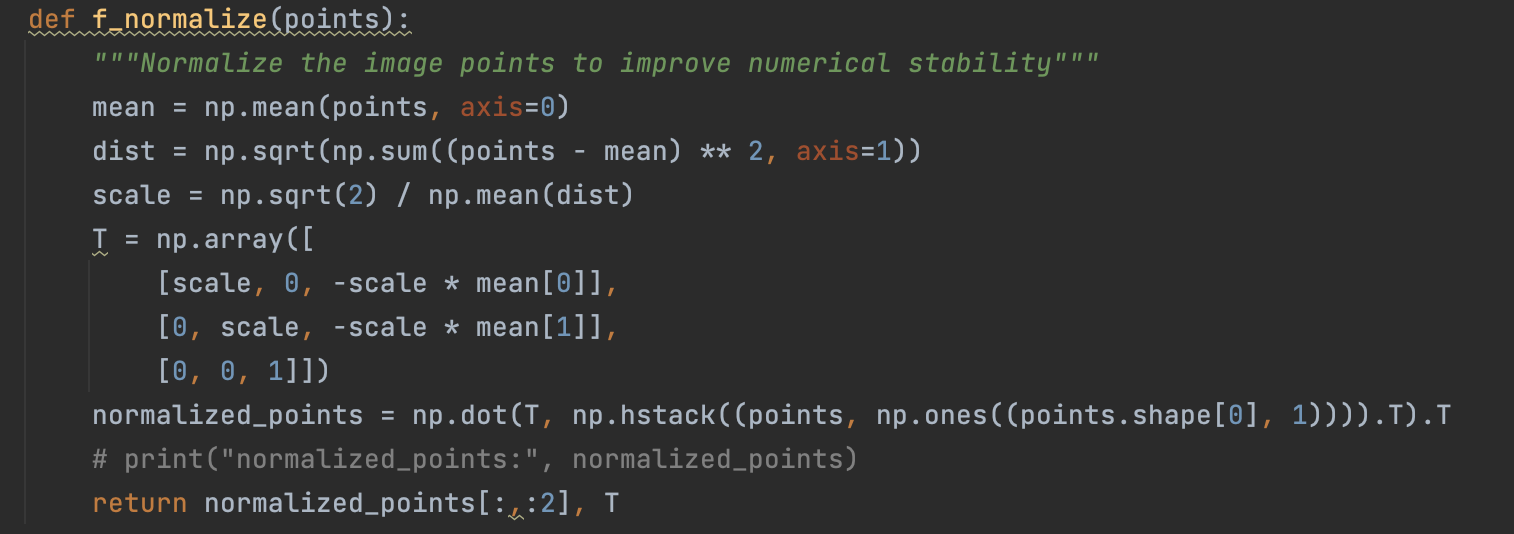
\includegraphics[width=0.4\linewidth]{fig/q2normalized _unction.png}
    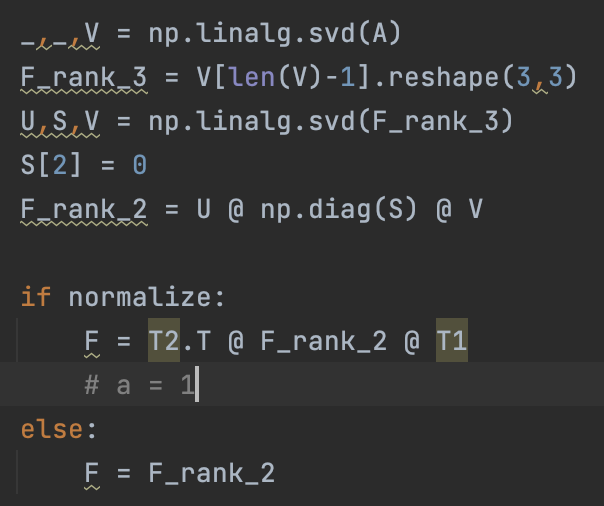
\includegraphics[width=0.4\linewidth]{fig/q2reconstruct.png}
\end{center}

The average geo distance of noramlized and unnormalized is shown as follows:

F with normalization average geo distance: 0.016614733966832926

F without normalization average geo distance: 0.02320321394917297

\paragraph{Question 3 (RANSAC) [3 pts]:} Here you will be modifying ``fundamental.py". Your task is to implement RANSAC to find the fundamental matrix between two cameras. Please report the average geometric distance based on your estimated fundamental matrix, given 1, 100, and 10000 iterations of RANSAC. Please also visualize the inliers with your best estimated fundamental matrix in your solution for both images (we provide a visualization function). In your PDF, please also explain why we do not perform SVD or do a least-squares over all the matched key points. 

\textbf{Answer: } When I set the inlier threshold as $0.01$, the average geometrix estimation and images of inliers are shown as follows:

num iterations: 1; avg geo dis with best F: 0.020305667672022593;

num iterations: 100; avg geo dis with best F: 0.024475027314097675;

num iterations: 10000; avg geo dis with best F: 0.008811086280057676;

Pictures shown from left to right is iterations of 1, 100 and 10000.
\begin{center}
    \small
    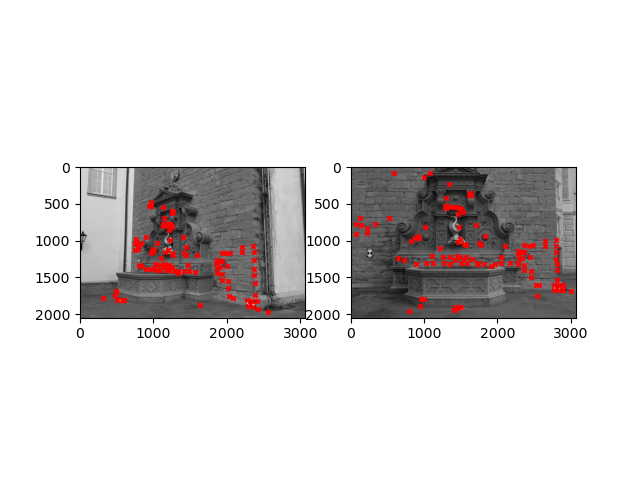
\includegraphics[width=0.3\linewidth]{fig/q3threshold0.01iter1.png}
    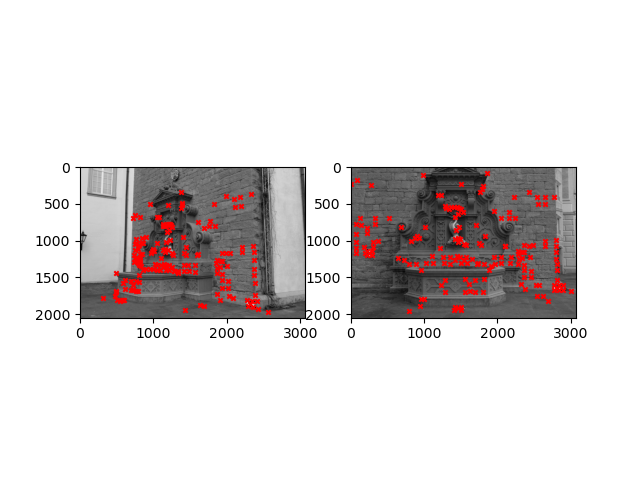
\includegraphics[width=0.3\linewidth]{fig/q3threshold0.01iter10.png}
    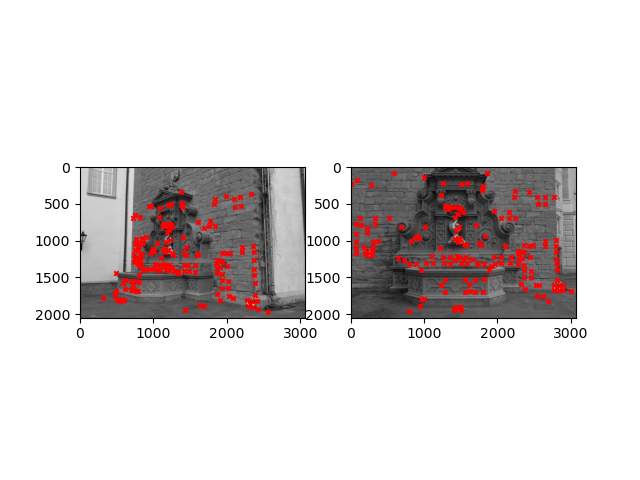
\includegraphics[width=0.3\linewidth]{fig/q3threshold0.01iter100.png}
\end{center}
When I set the inlier threshold as $0.1$, the average geometrix estimation and images of inliers are shown as follows:

num iterations: 1; avg geo dis with best F: 0.03472263464621629;

num iterations: 100; avg geo dis with best F: 0.016629860172547146;

num iterations: 10000; avg geo dis with best F: 0.015011251388708848;

Pictures shown from left to right is iterations of 1, 100 and 10000.
\begin{center}
    \small
    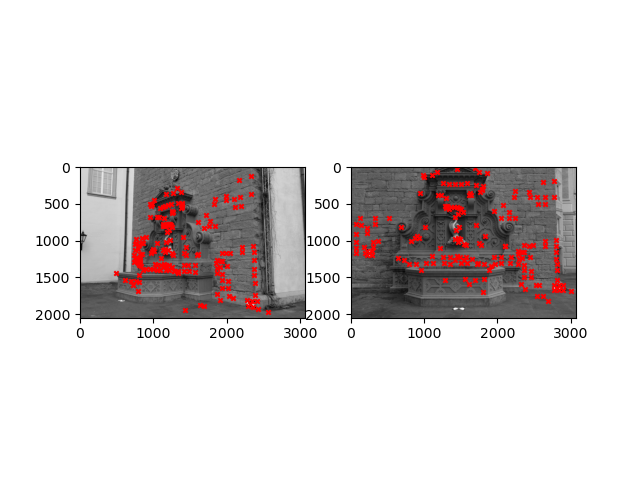
\includegraphics[width=0.3\linewidth]{fig/q3threshold0.1iter1.png}
    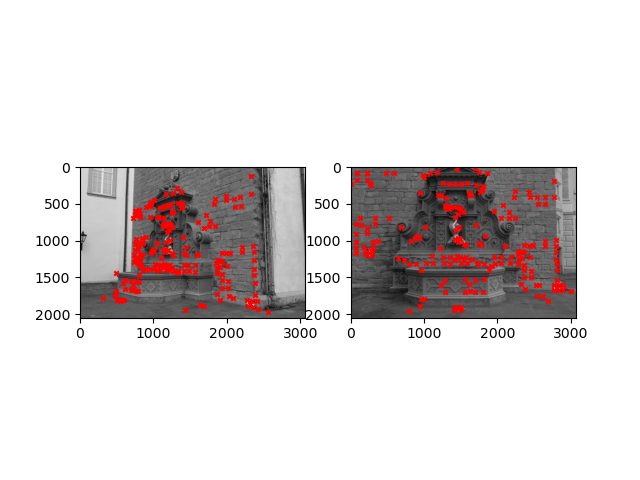
\includegraphics[width=0.3\linewidth]{fig/q3threshold0.1iter10.png}
    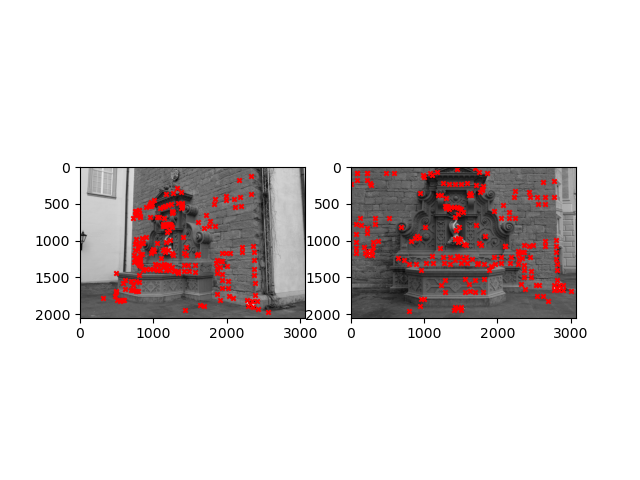
\includegraphics[width=0.3\linewidth]{fig/q3threshold0.1iter100.png}
\end{center}

The reason why we do not perform SVD or do least-squares over all matched key points is that the presence of outliers can significantly affect the accuracy of the estimate. If we use SVD or least squares directly to all matched, the outliers will affect the estimation. However, if we use the RANSAC, we can get rid of the affect of outliers by filter them out during the RANSAC.

\paragraph{Question 4 (Epipolar Line Visualization) [1 pt]:} Here you will be modifying ``fundamental.py". Please visualize the epipolar line for both images for your estimated F in Q2 and Q3. Here we do not provide you visualization code. To draw on images, cv2.line, cv2.circle are useful for plotting lines and circles. Check our Lecture 4 slides on Epipolar Geometry, to learn more about equation of epipolar line. This \href{https://web.stanford.edu/class/cs231a/course_notes/03-epipolar-geometry.pdf}{link} also gives a thorough review of epipolar geometry.

\textbf{Answer: } The output images of epipolar line for both images are shown as follows, The first row is of estimated F in Q2 and the second row is of estimated F in Q3. The left image is image 1 and the right image is image2,
\begin{center}
    \small
    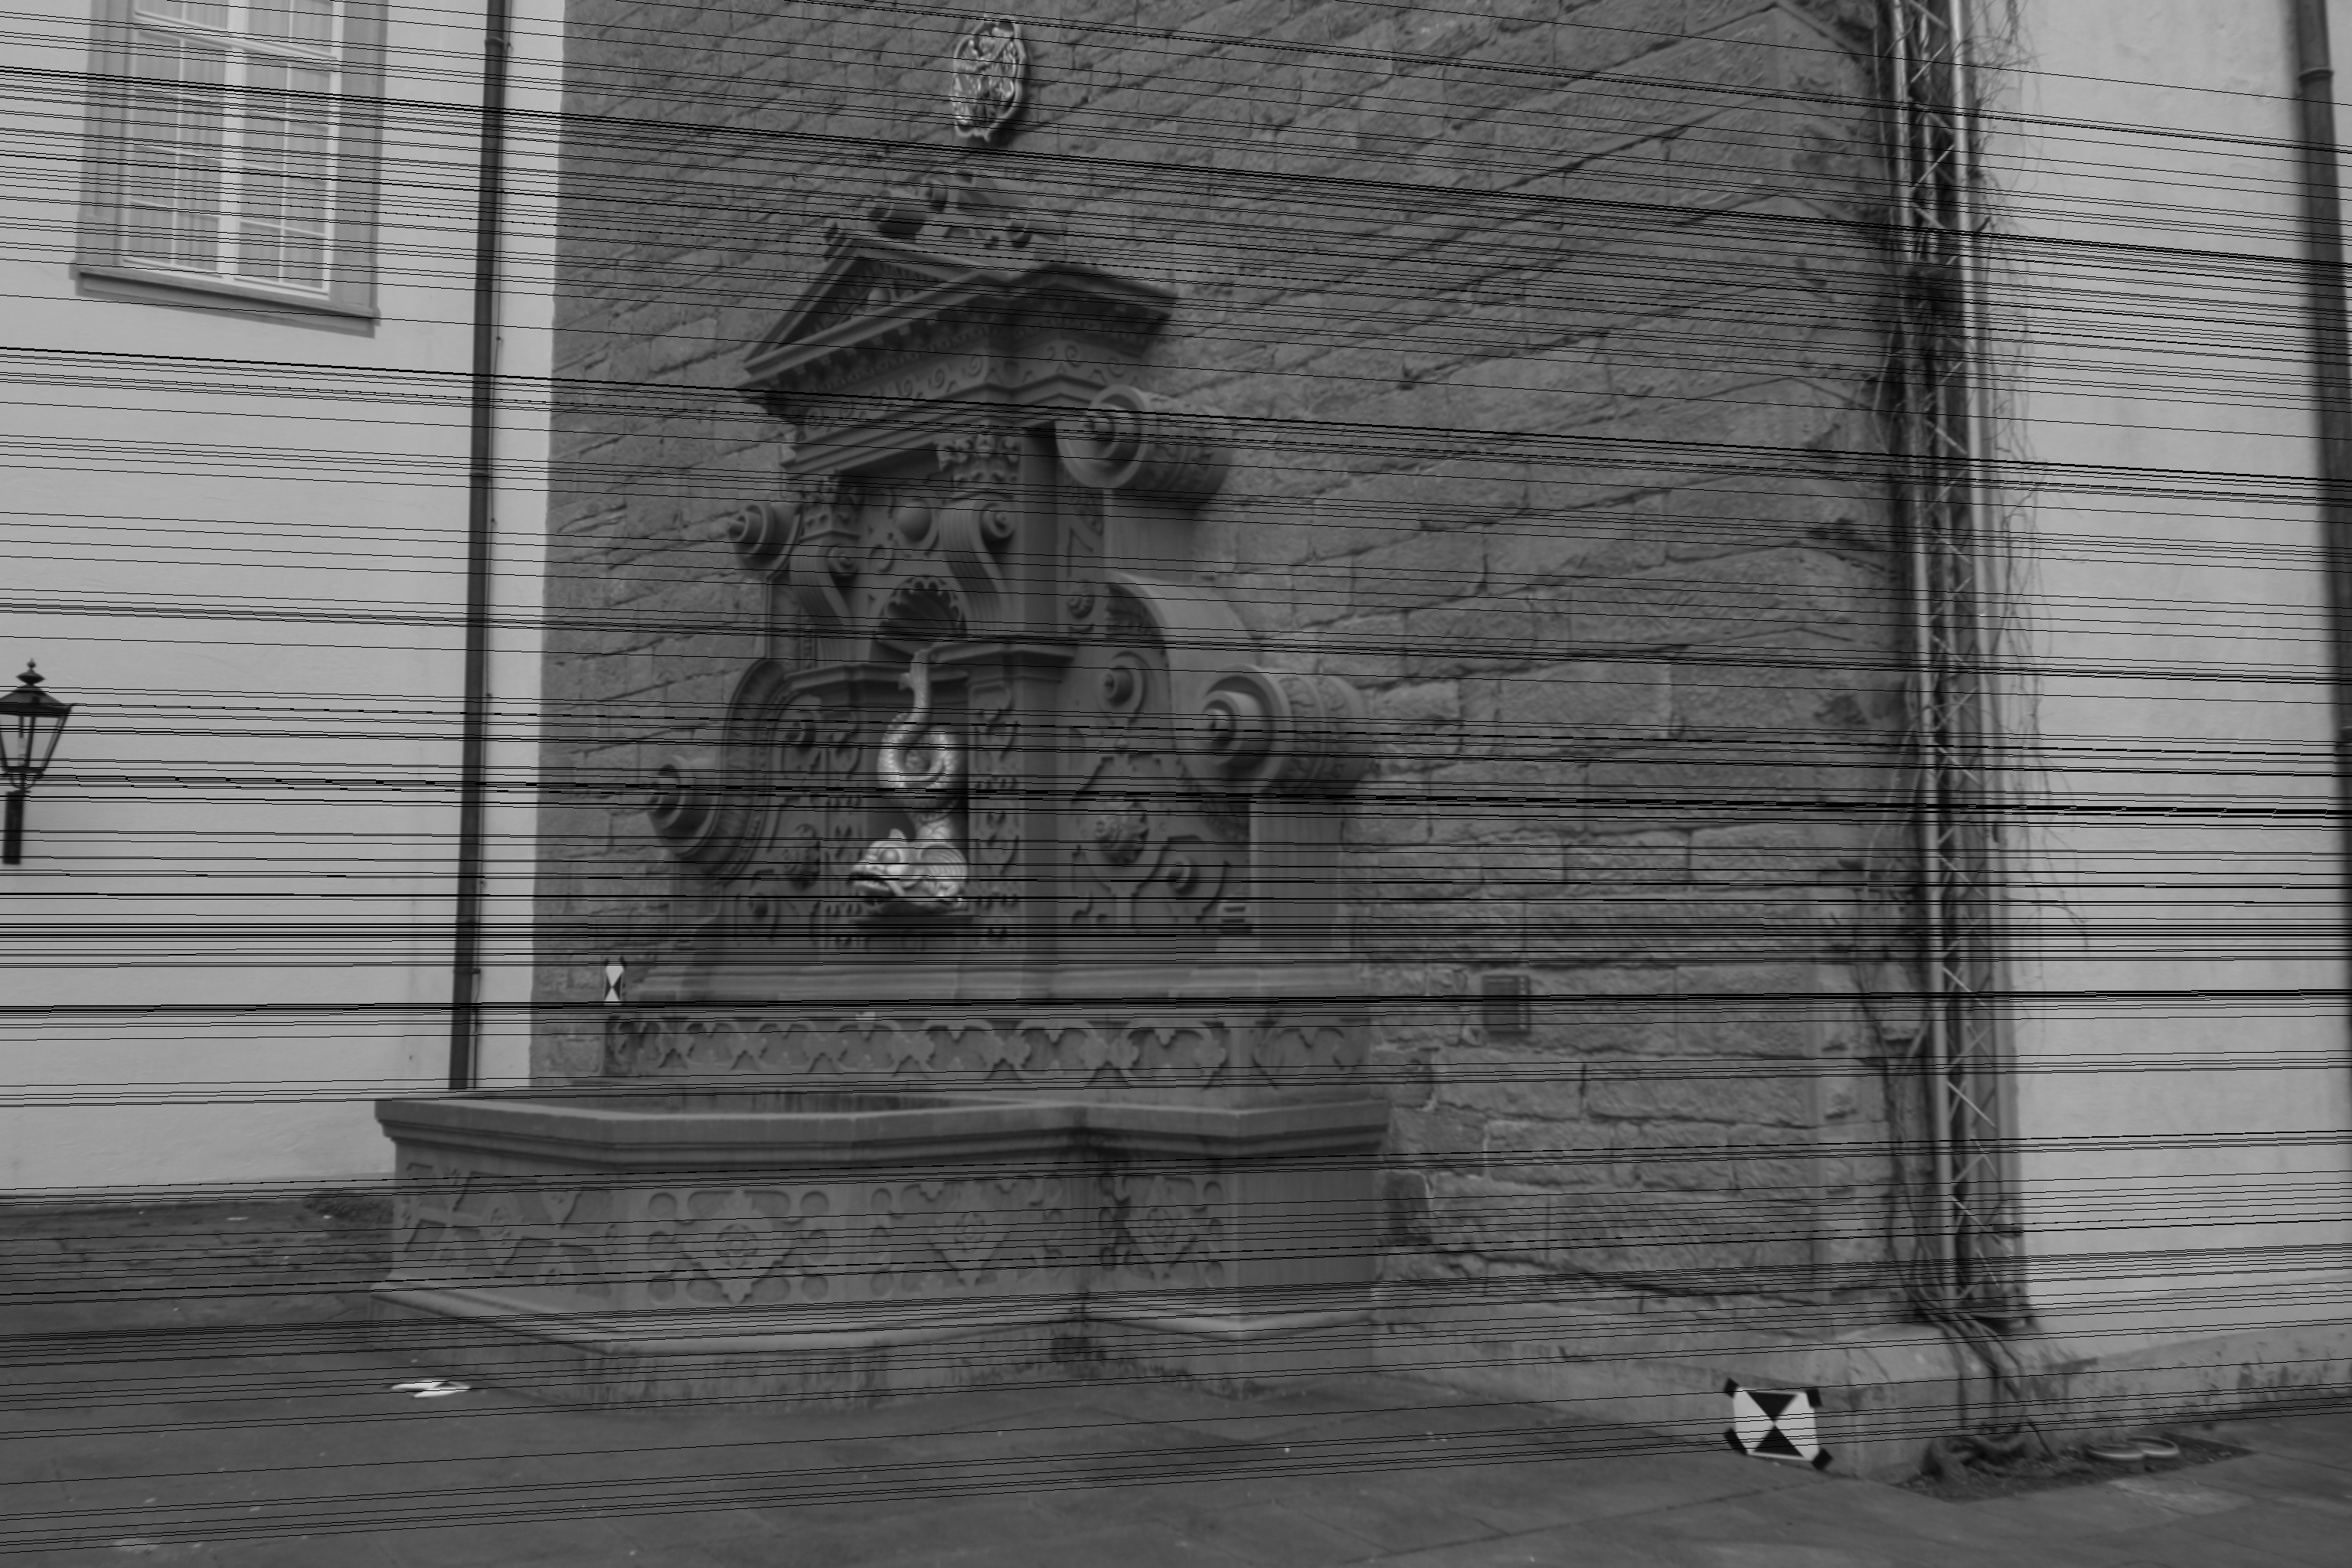
\includegraphics[width=0.4\linewidth]{fig/Q4_Q2Image1.png}
    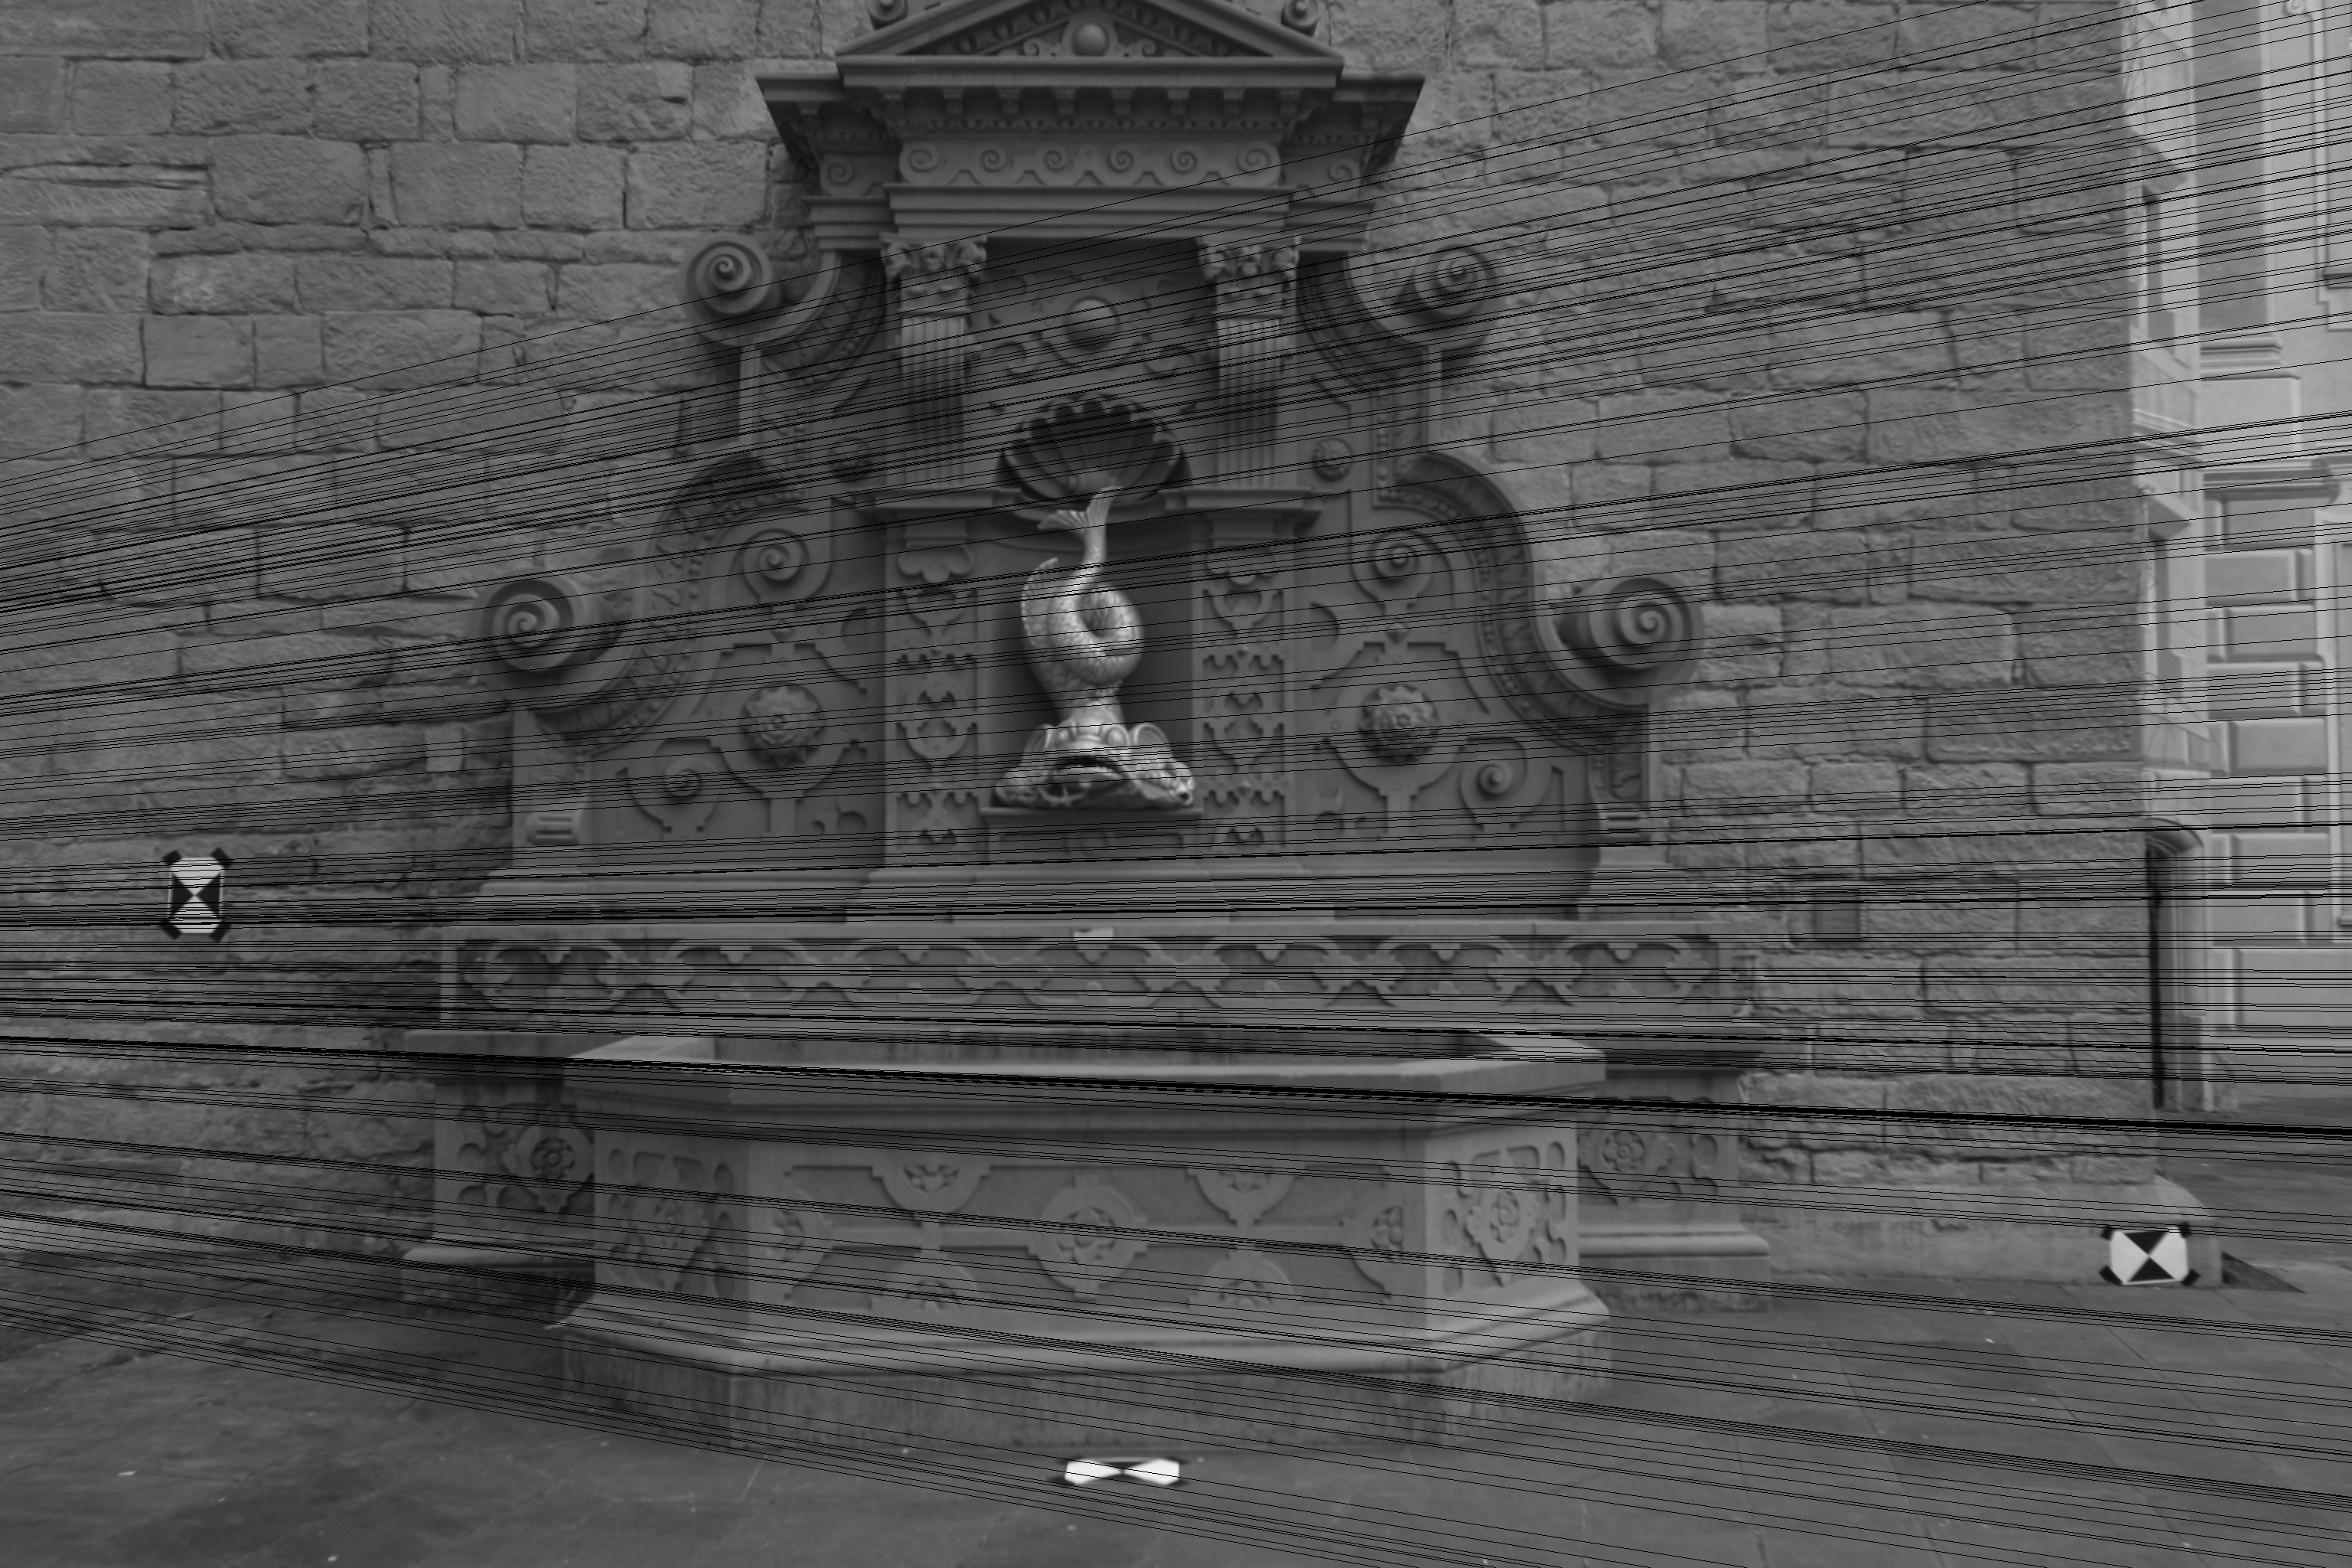
\includegraphics[width=0.4\linewidth]{fig/Q4_Q2img2.png}
\end{center}
\begin{center}
    \small
    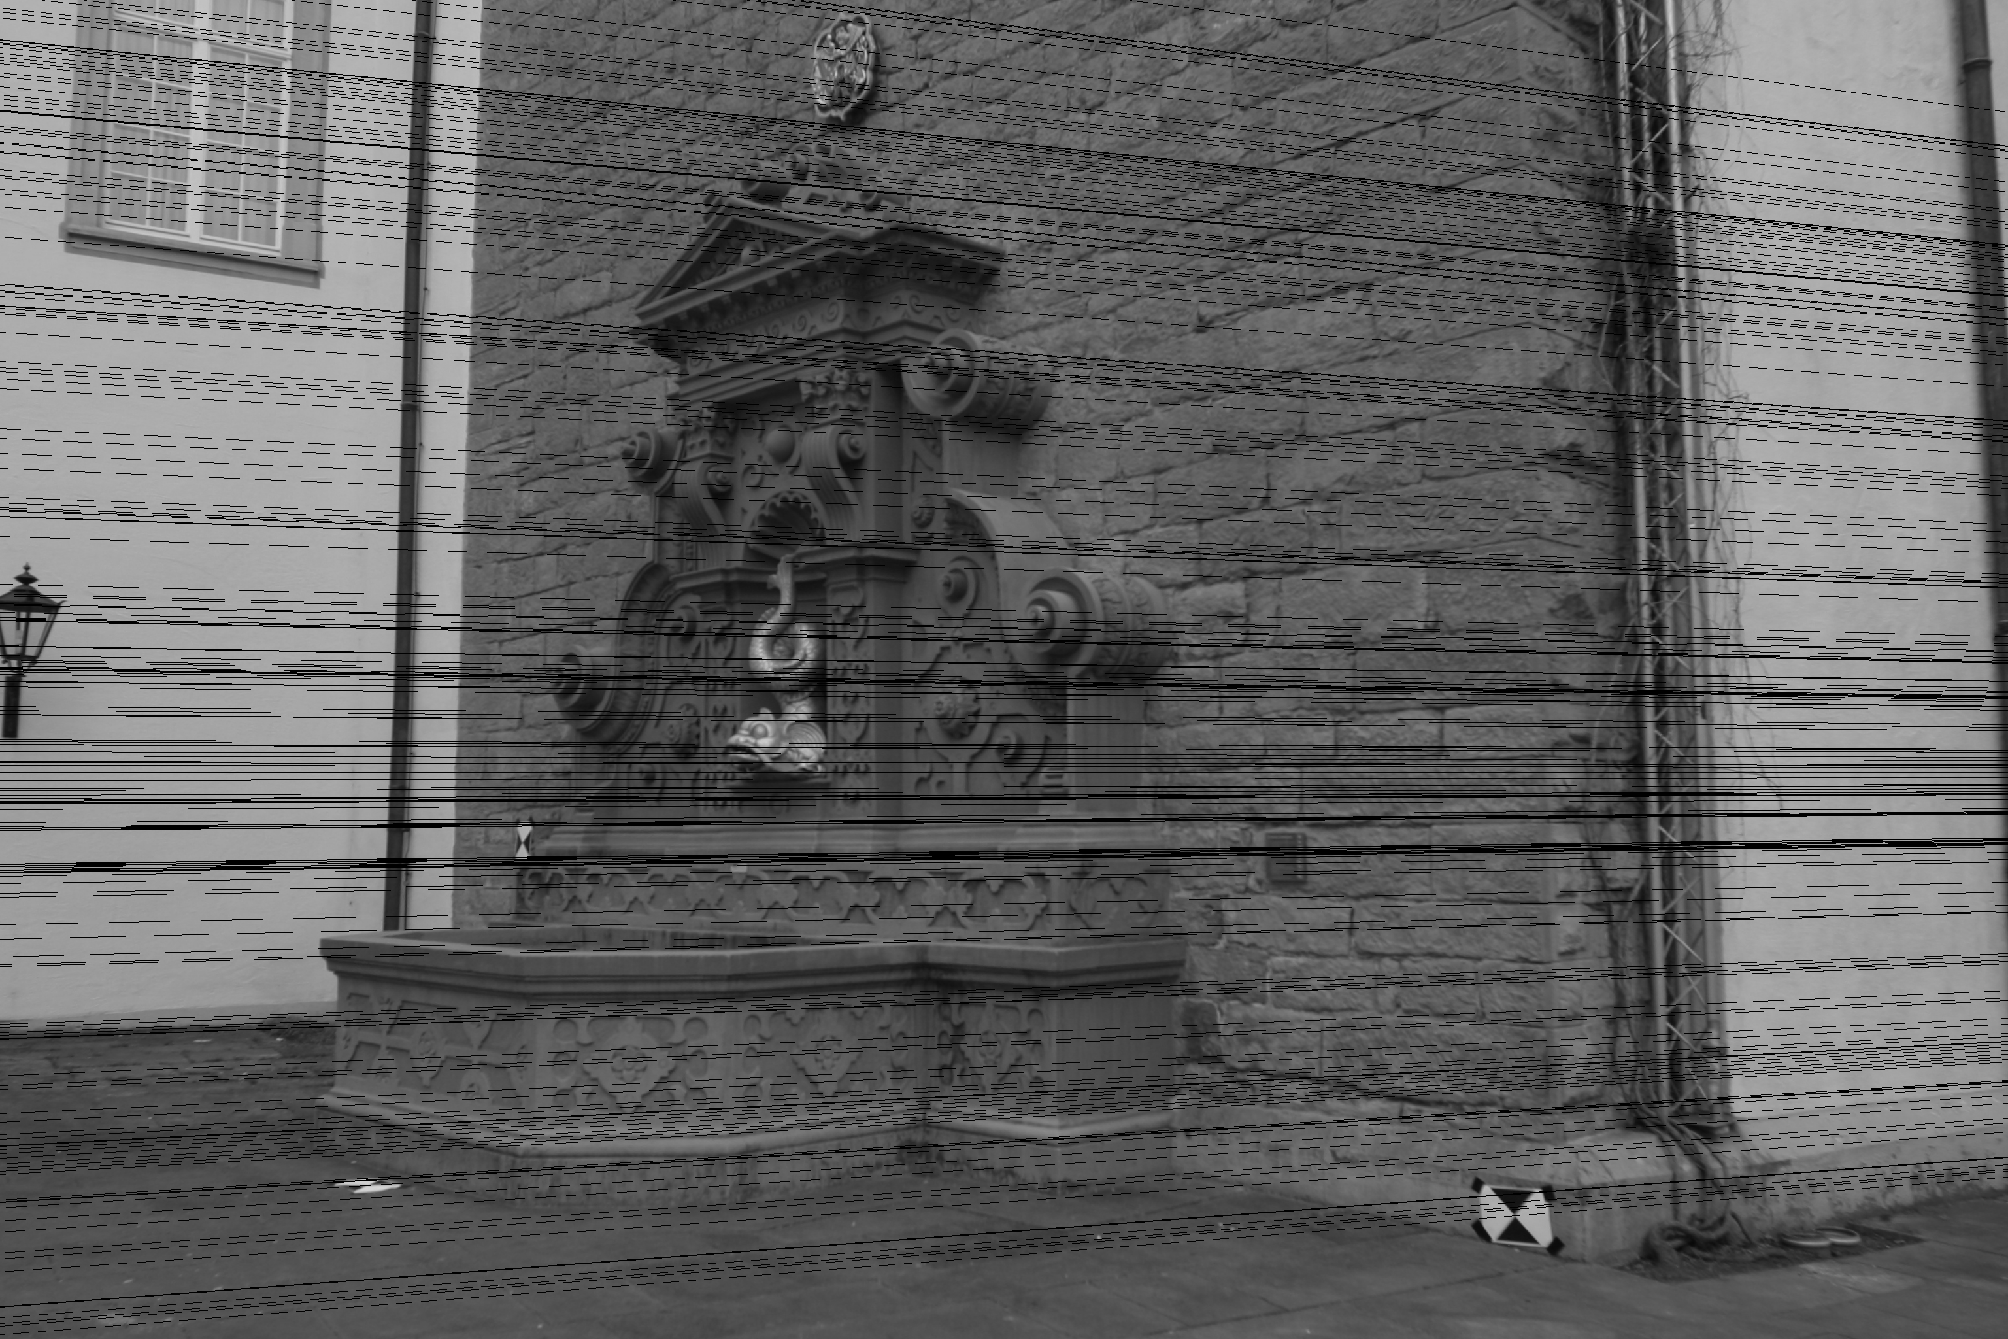
\includegraphics[width=0.4\linewidth]{fig/Q4_Q3img1.png}
    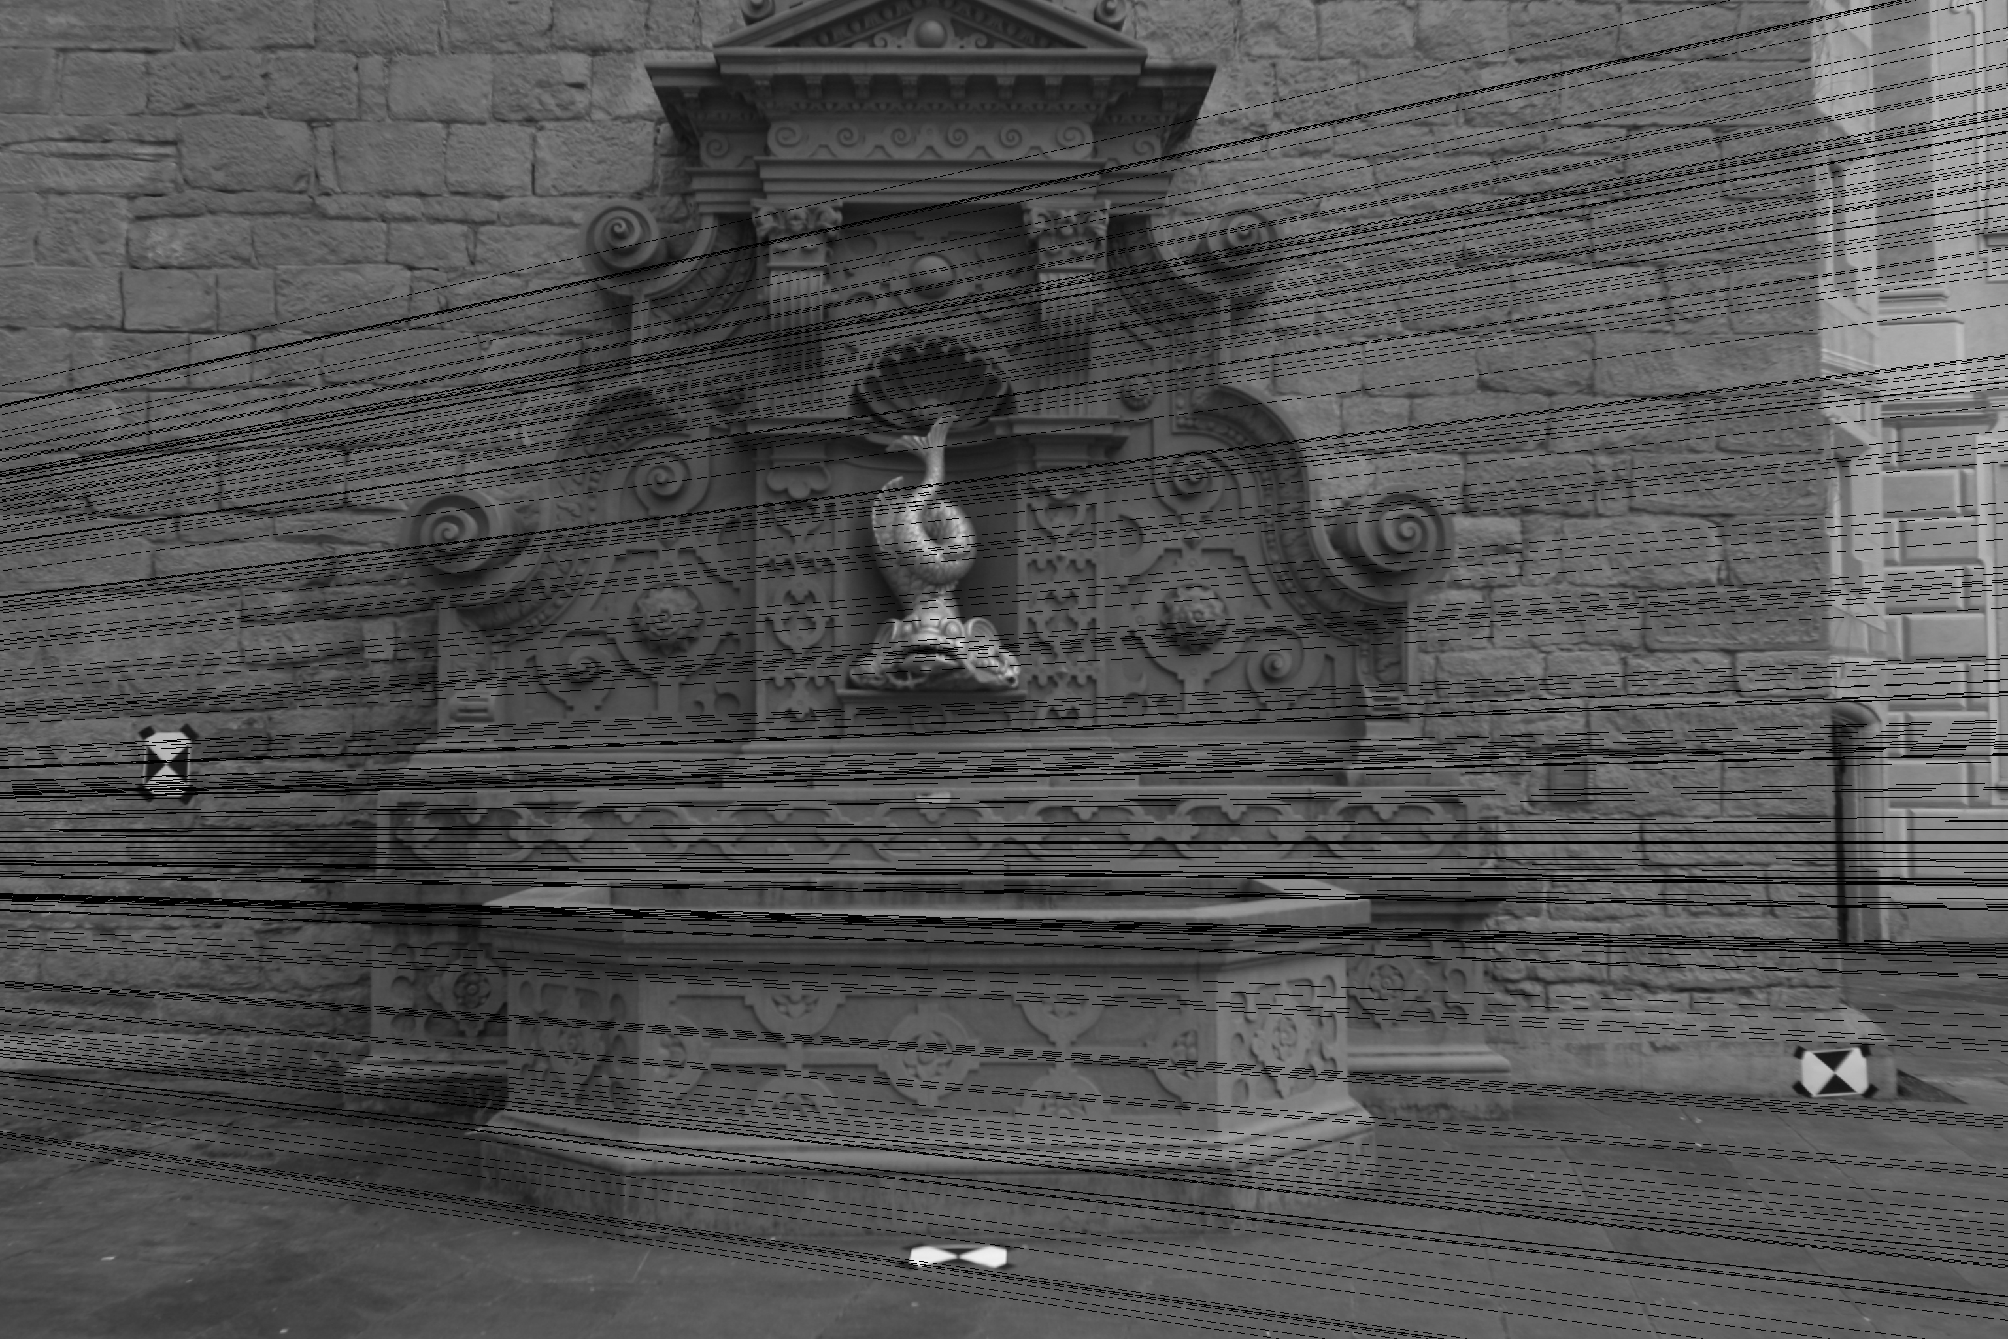
\includegraphics[width=0.4\linewidth]{fig/Q4_Q3Img2.png}
\end{center}
The visualize function is shown as follows:
\begin{center}
    \small
    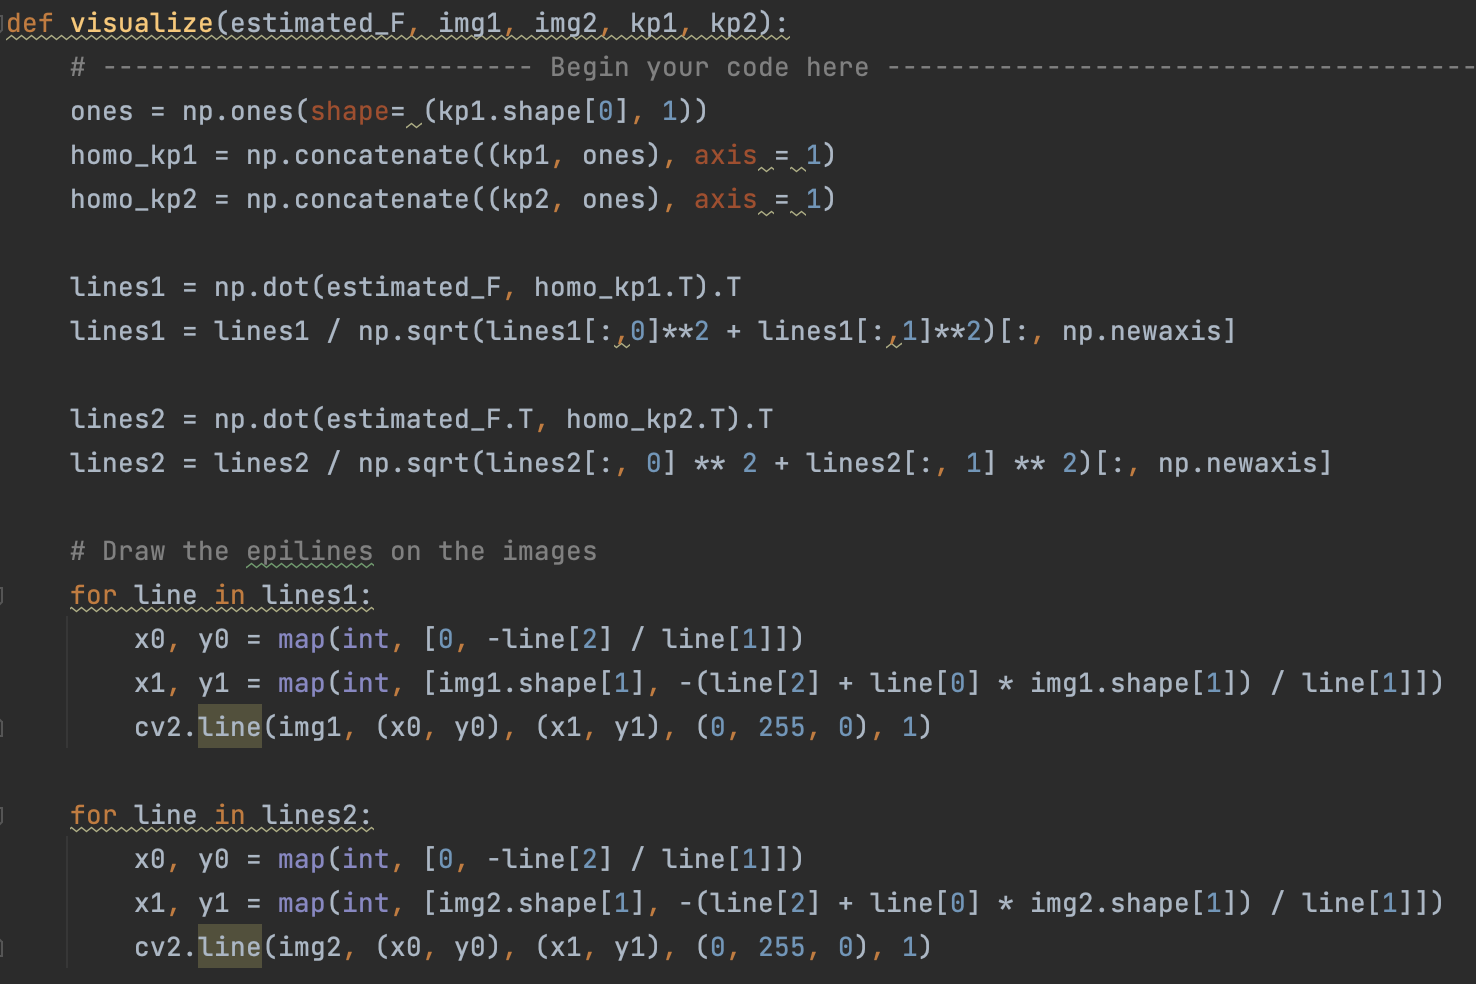
\includegraphics[width=0.4\linewidth]{fig/Q4visualize.png}
\end{center}

\section*{Unprojection} 
After solving relative poses between our two cameras, now we will move from 2d to 3d space.

\paragraph{Question 5 (Triangulation) [3 pts]:}
Here you will be modifying ``triangulation.py". You are given keypoint matching between two images, together with the camera intrinsic and extrinsic matrix. Your task is to perform triangulation to restore the 3D coordinates of the key points. In your PDF, please visualize the 3d points and camera poses in 3D from three different viewing perspectives. 

\textbf{Answer: } Here is the images of 3d points and two camera pose.
\begin{center}
    \small
    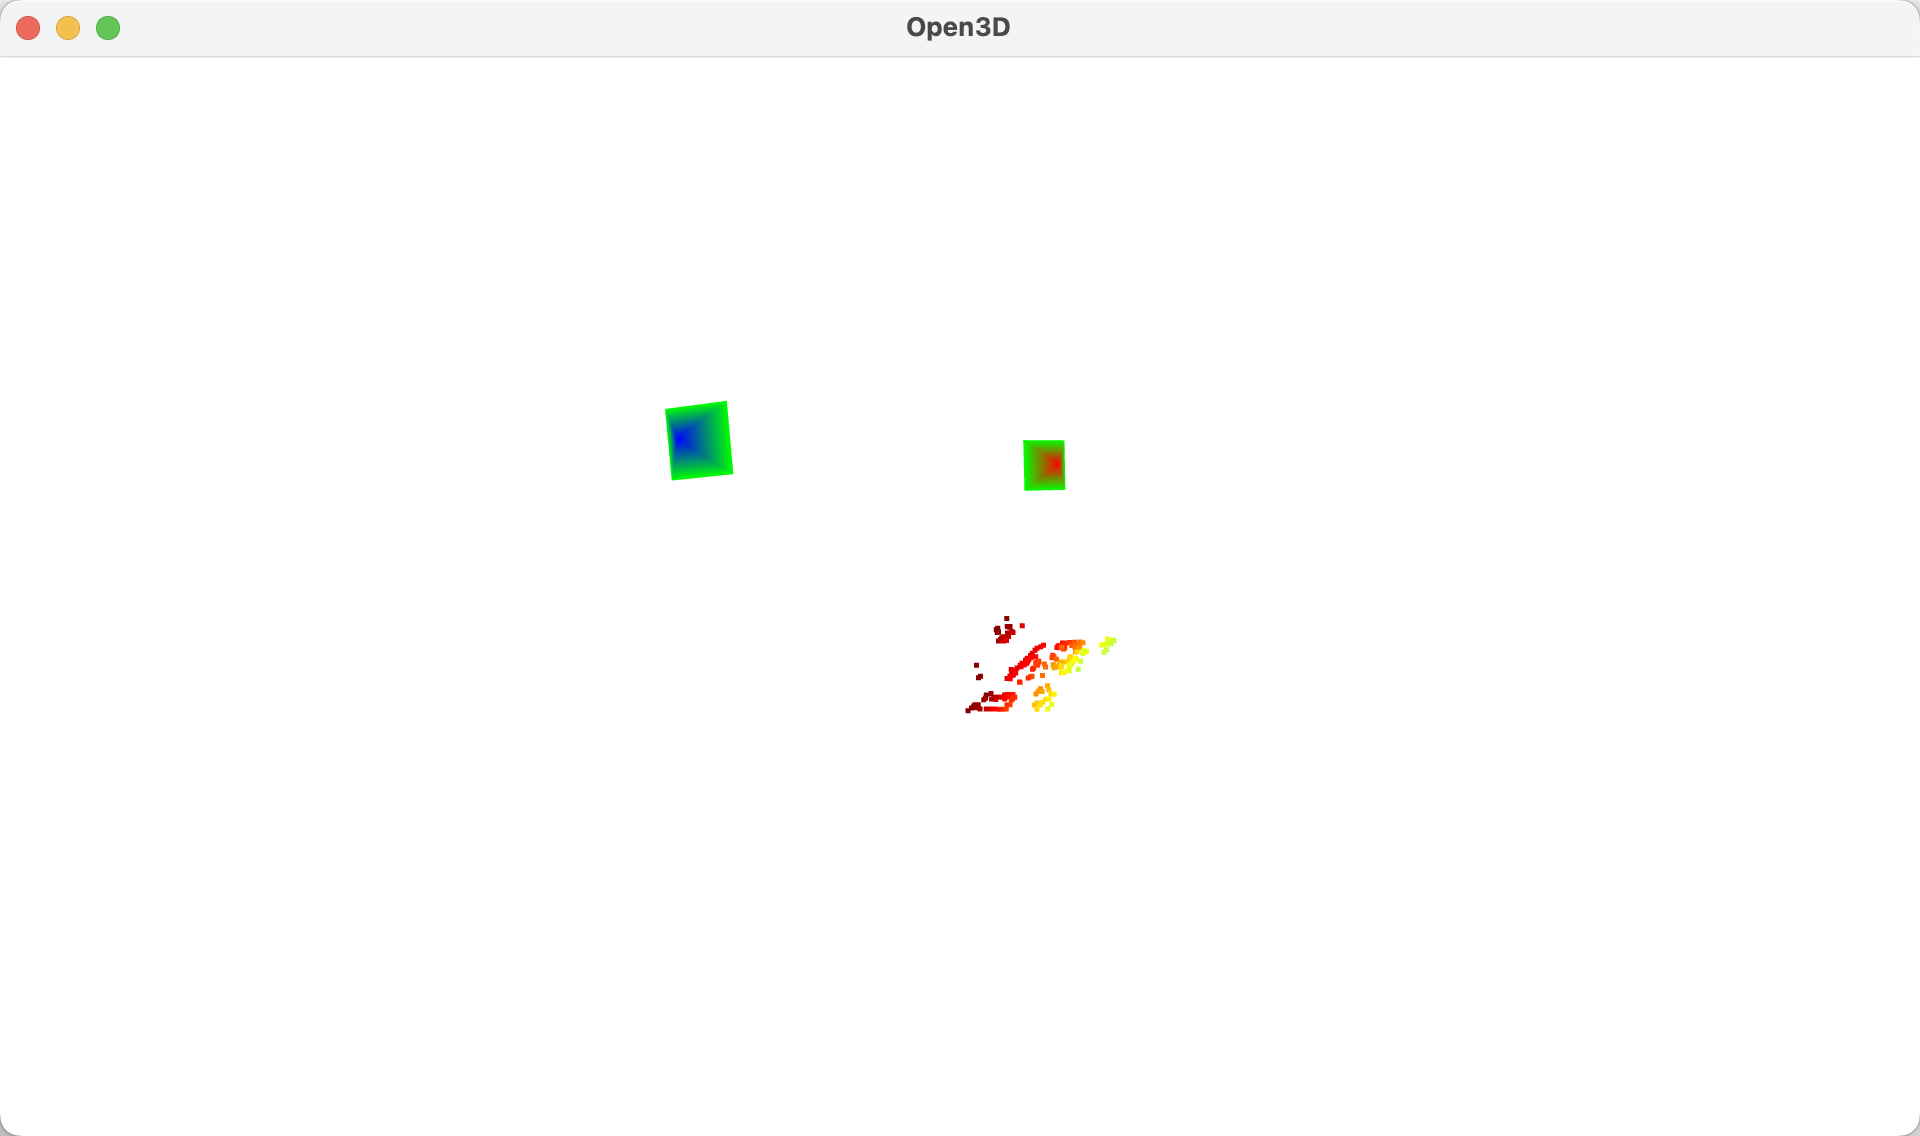
\includegraphics[width=0.3\linewidth]{fig/q5img1.png}
    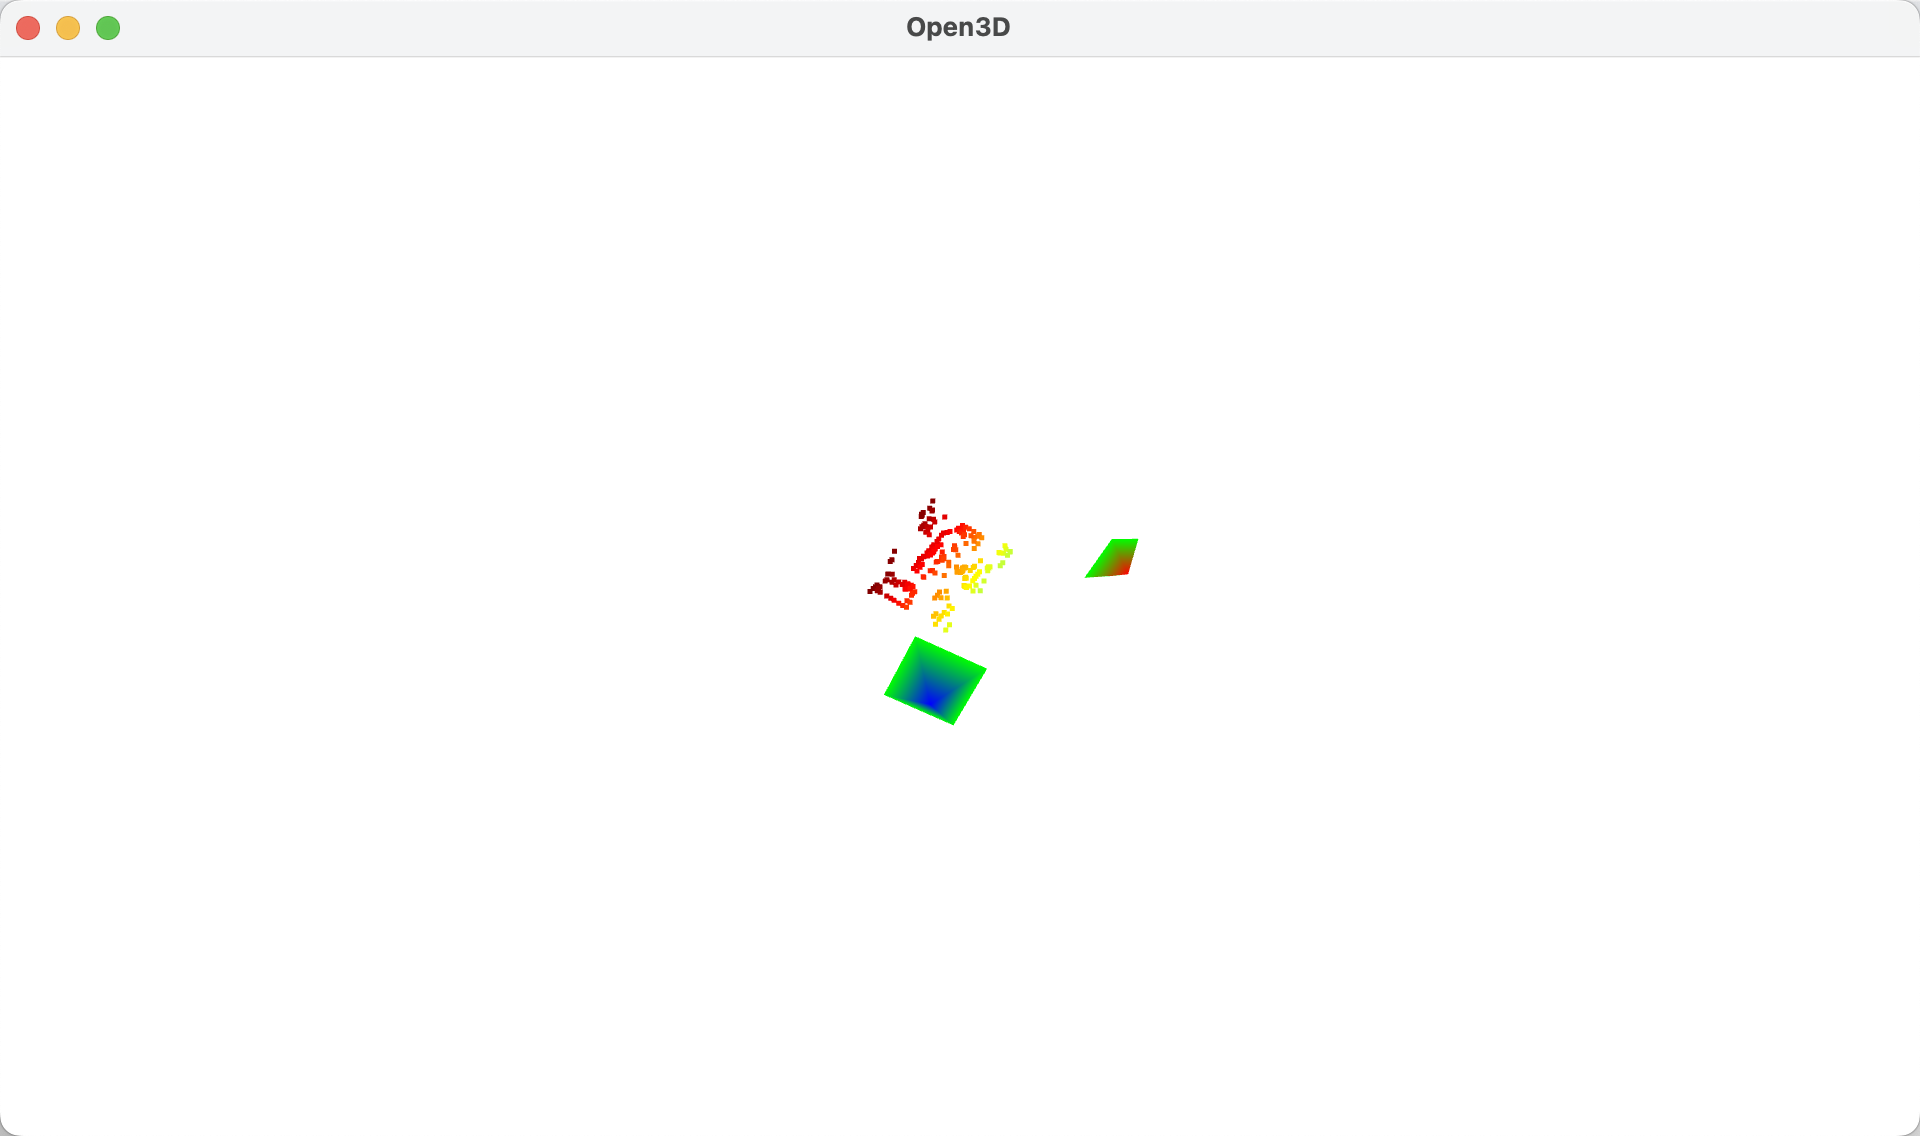
\includegraphics[width=0.3\linewidth]{fig/q5img2.png}
    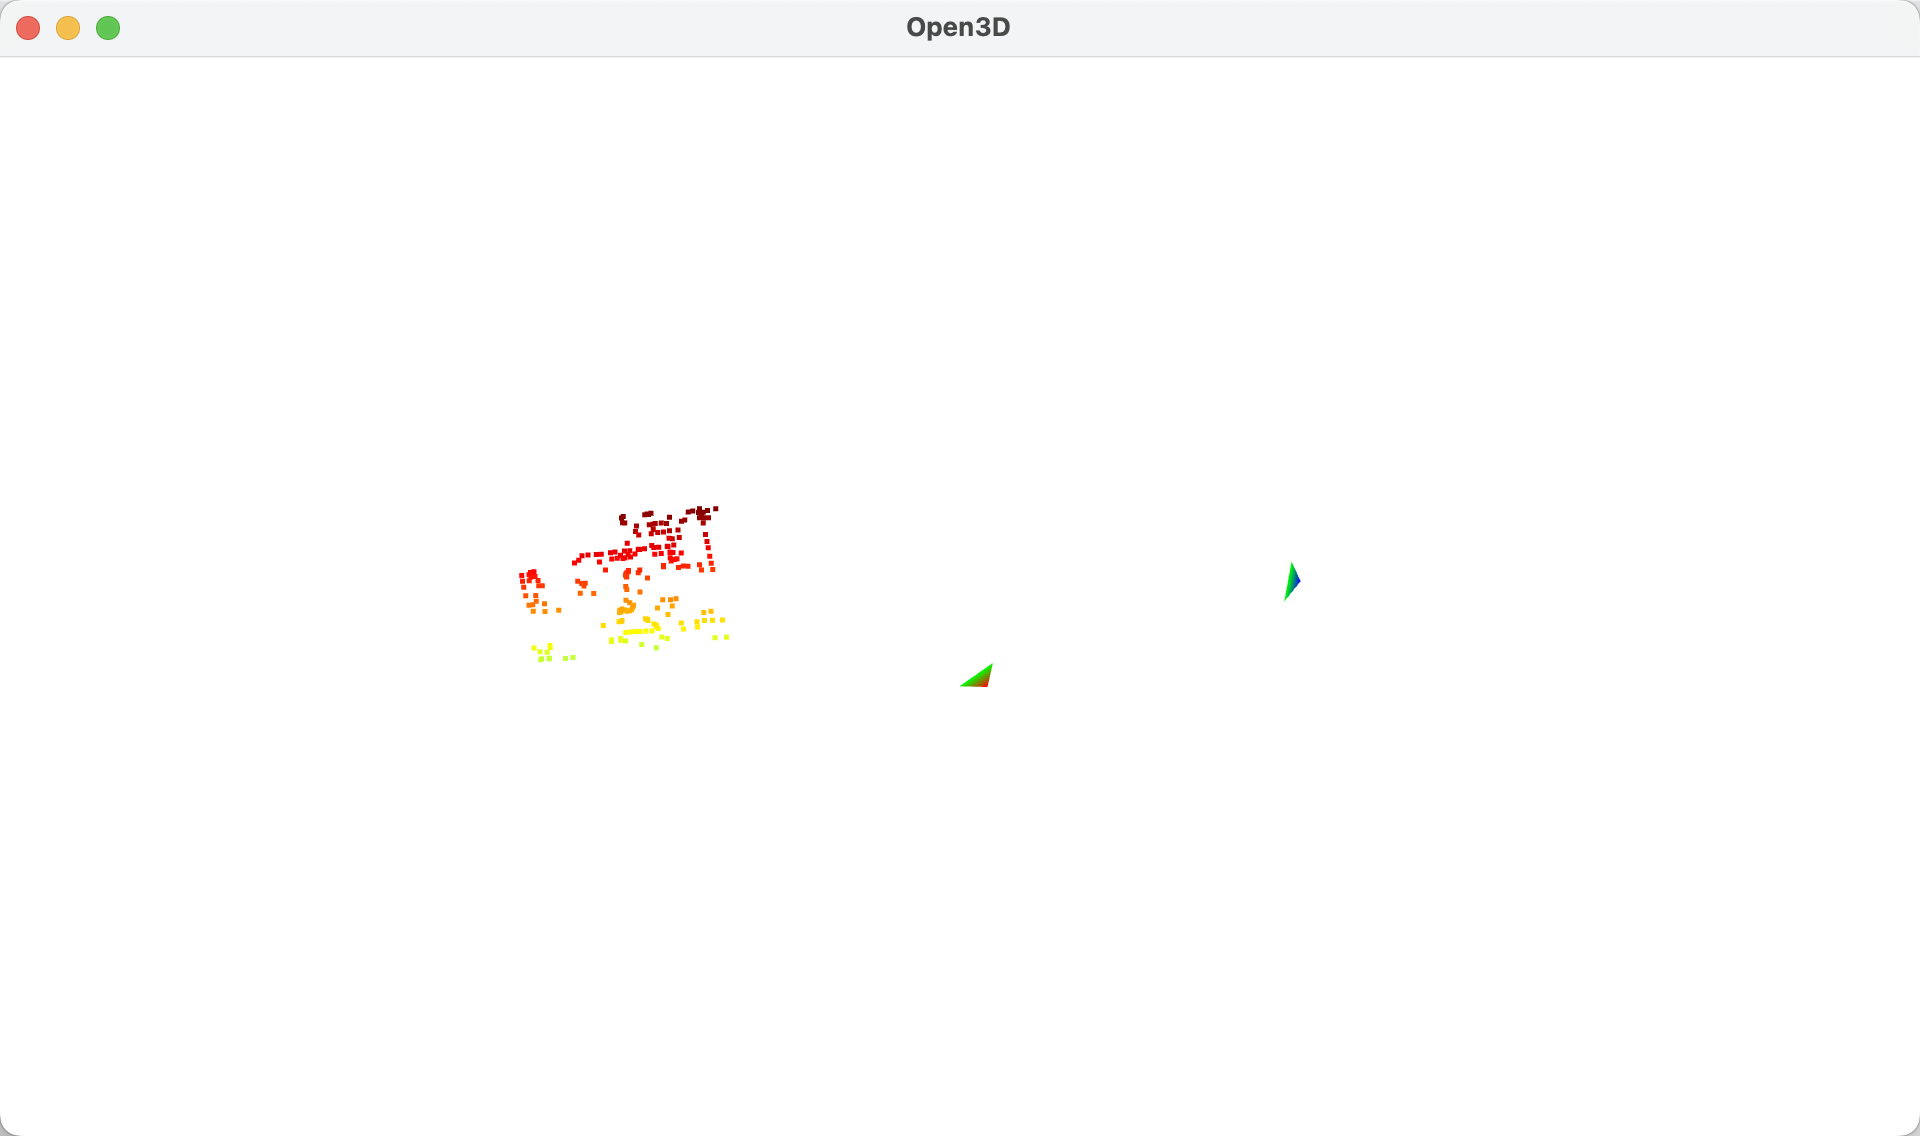
\includegraphics[width=0.3\linewidth]{fig/q5img4.png}
\end{center}

The pyramid with red vertex is the camera1 while the pyramid with blue vertex is camera2. I set the init pyramid vertices coordinates as follows:

\[vertices = 
\left[
\begin{array}{ccc}
    0 & 0 & 0 \\
    -1 & 1 & -1 \\
    -1 & 1 & 1 \\
    -1 & -1 & 1 \\
    -1 & -1 & -1
\end{array}
\right]
\]

One thing that should be noticed is that I use the pyramid as a sign of camera, however, it does not means that the FOV is same as the pyramid. There are some key function that I used to visualize 3d points and camera, shows as follows. The left image is the way I create pyramid as the symbol of camera and the right image is for visualizing 3D-points(pcd) and camera poses.
\begin{center}
    \small
    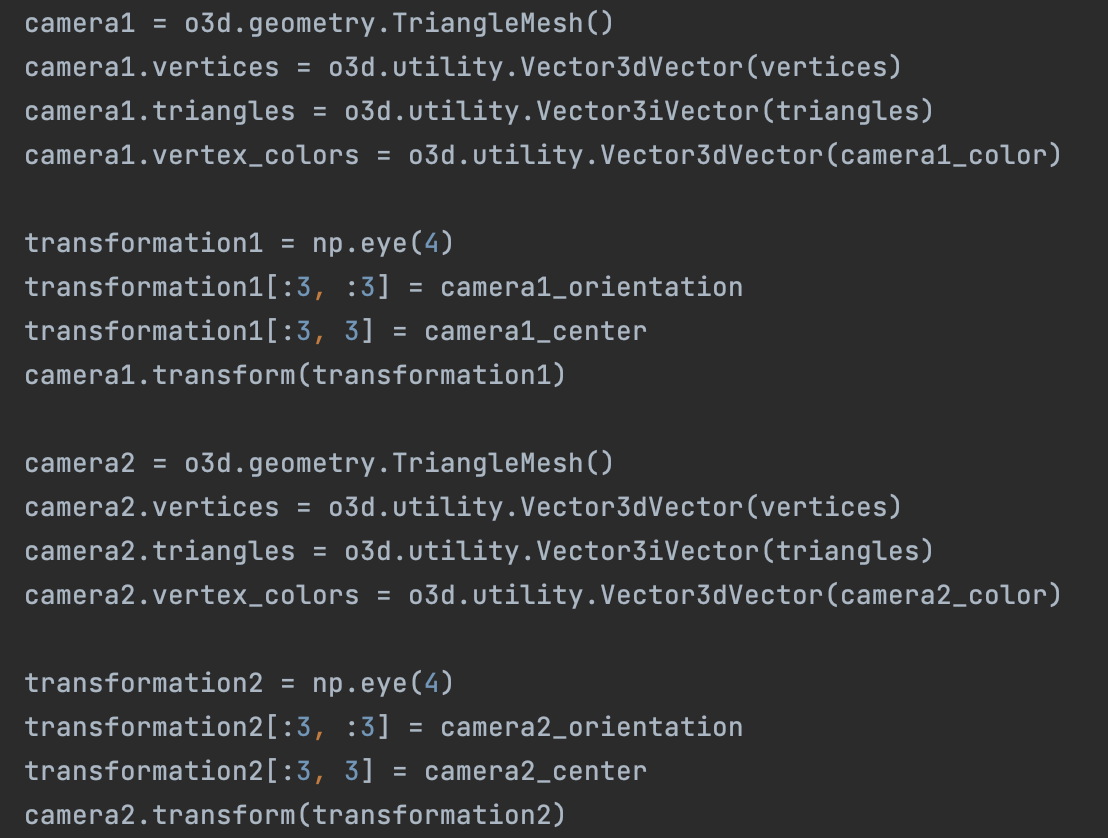
\includegraphics[width=0.3\linewidth]{fig/q5function1.png}
    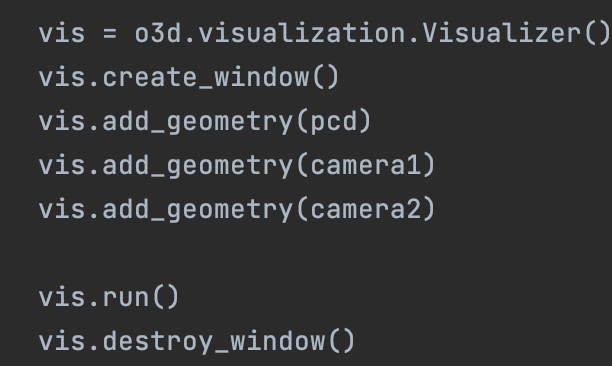
\includegraphics[width=0.3\linewidth]{fig/q5function2.png}
\end{center}

After all this DIY method, I realize there is a specific way to draw camera image in 3d space, which is geometry.LineSet.create camera visualization(). It's output is more clear and I think the camera pose is very accurate.
\begin{center}
    \small
    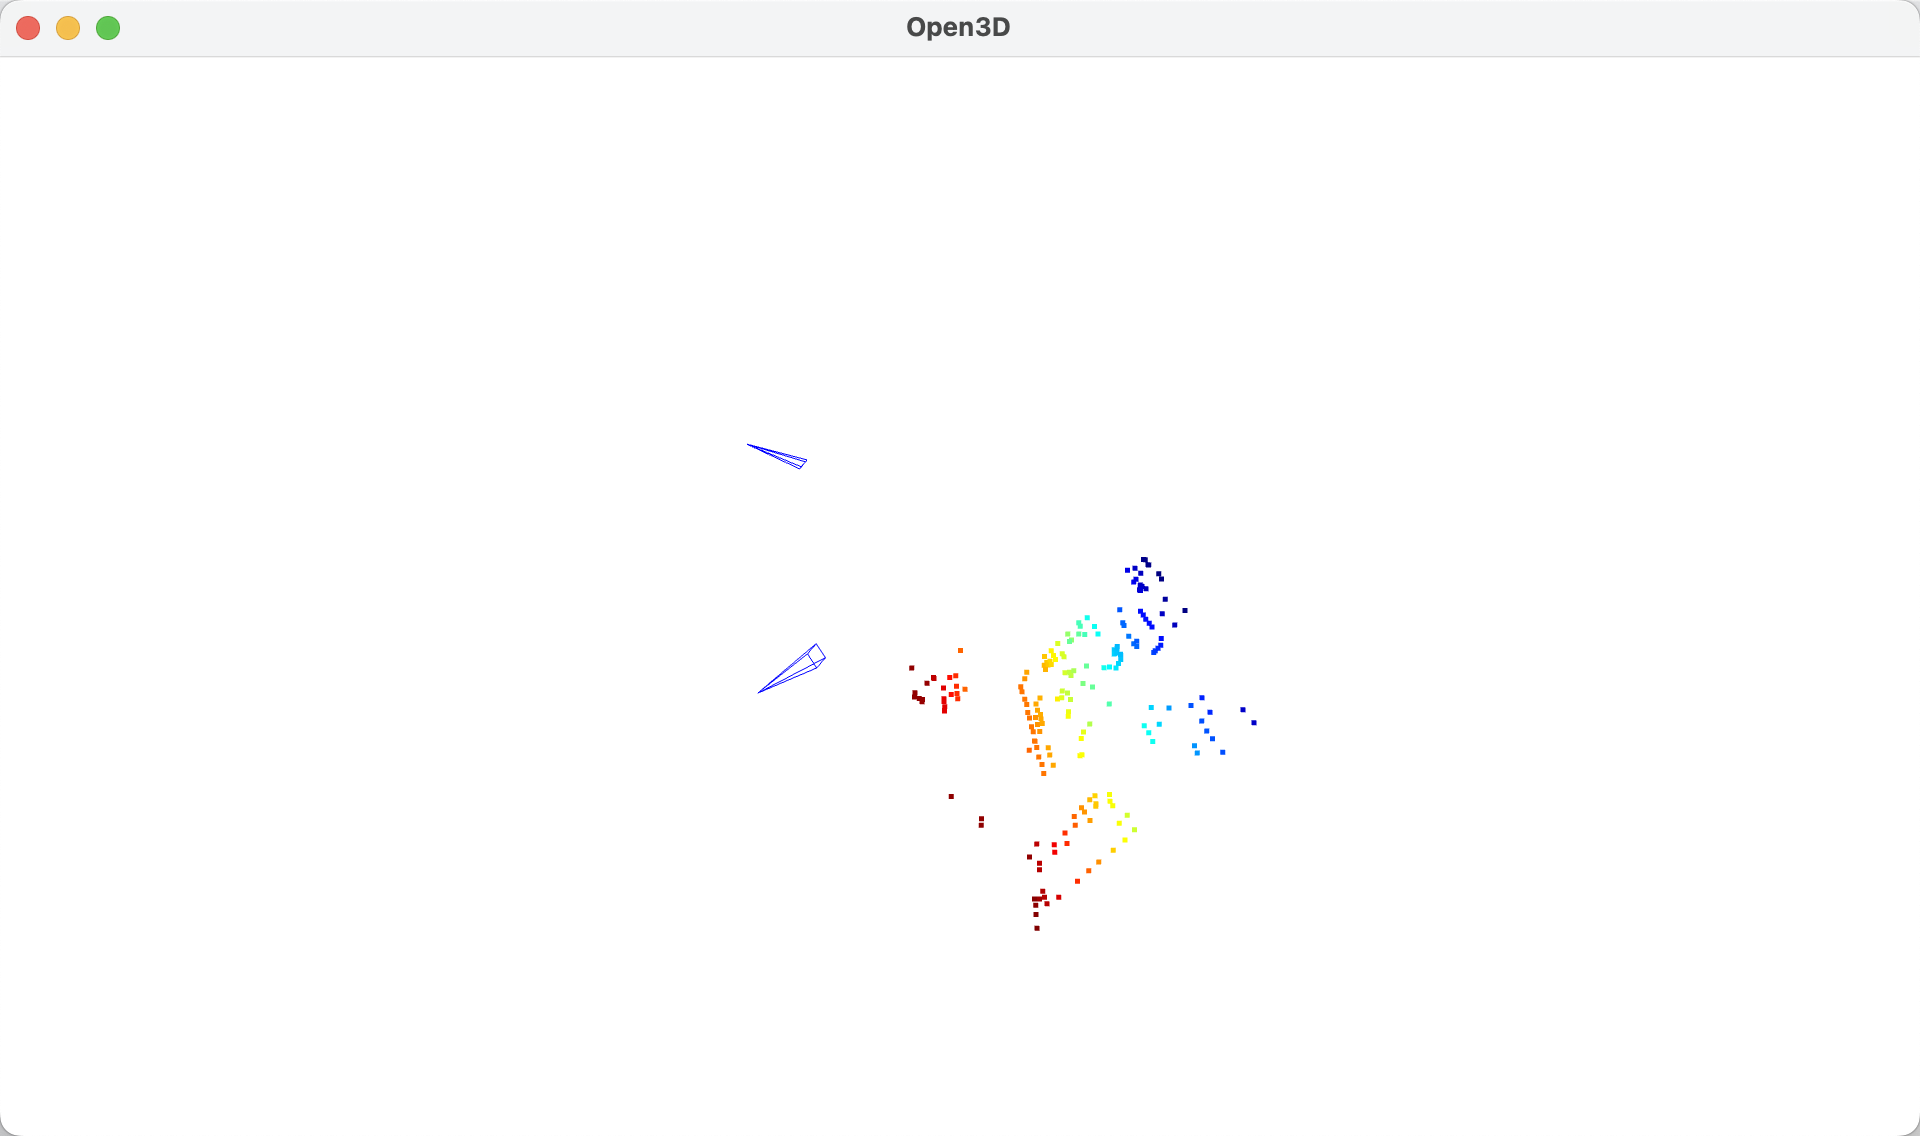
\includegraphics[width=0.3\linewidth]{fig/Q5right1.png}
    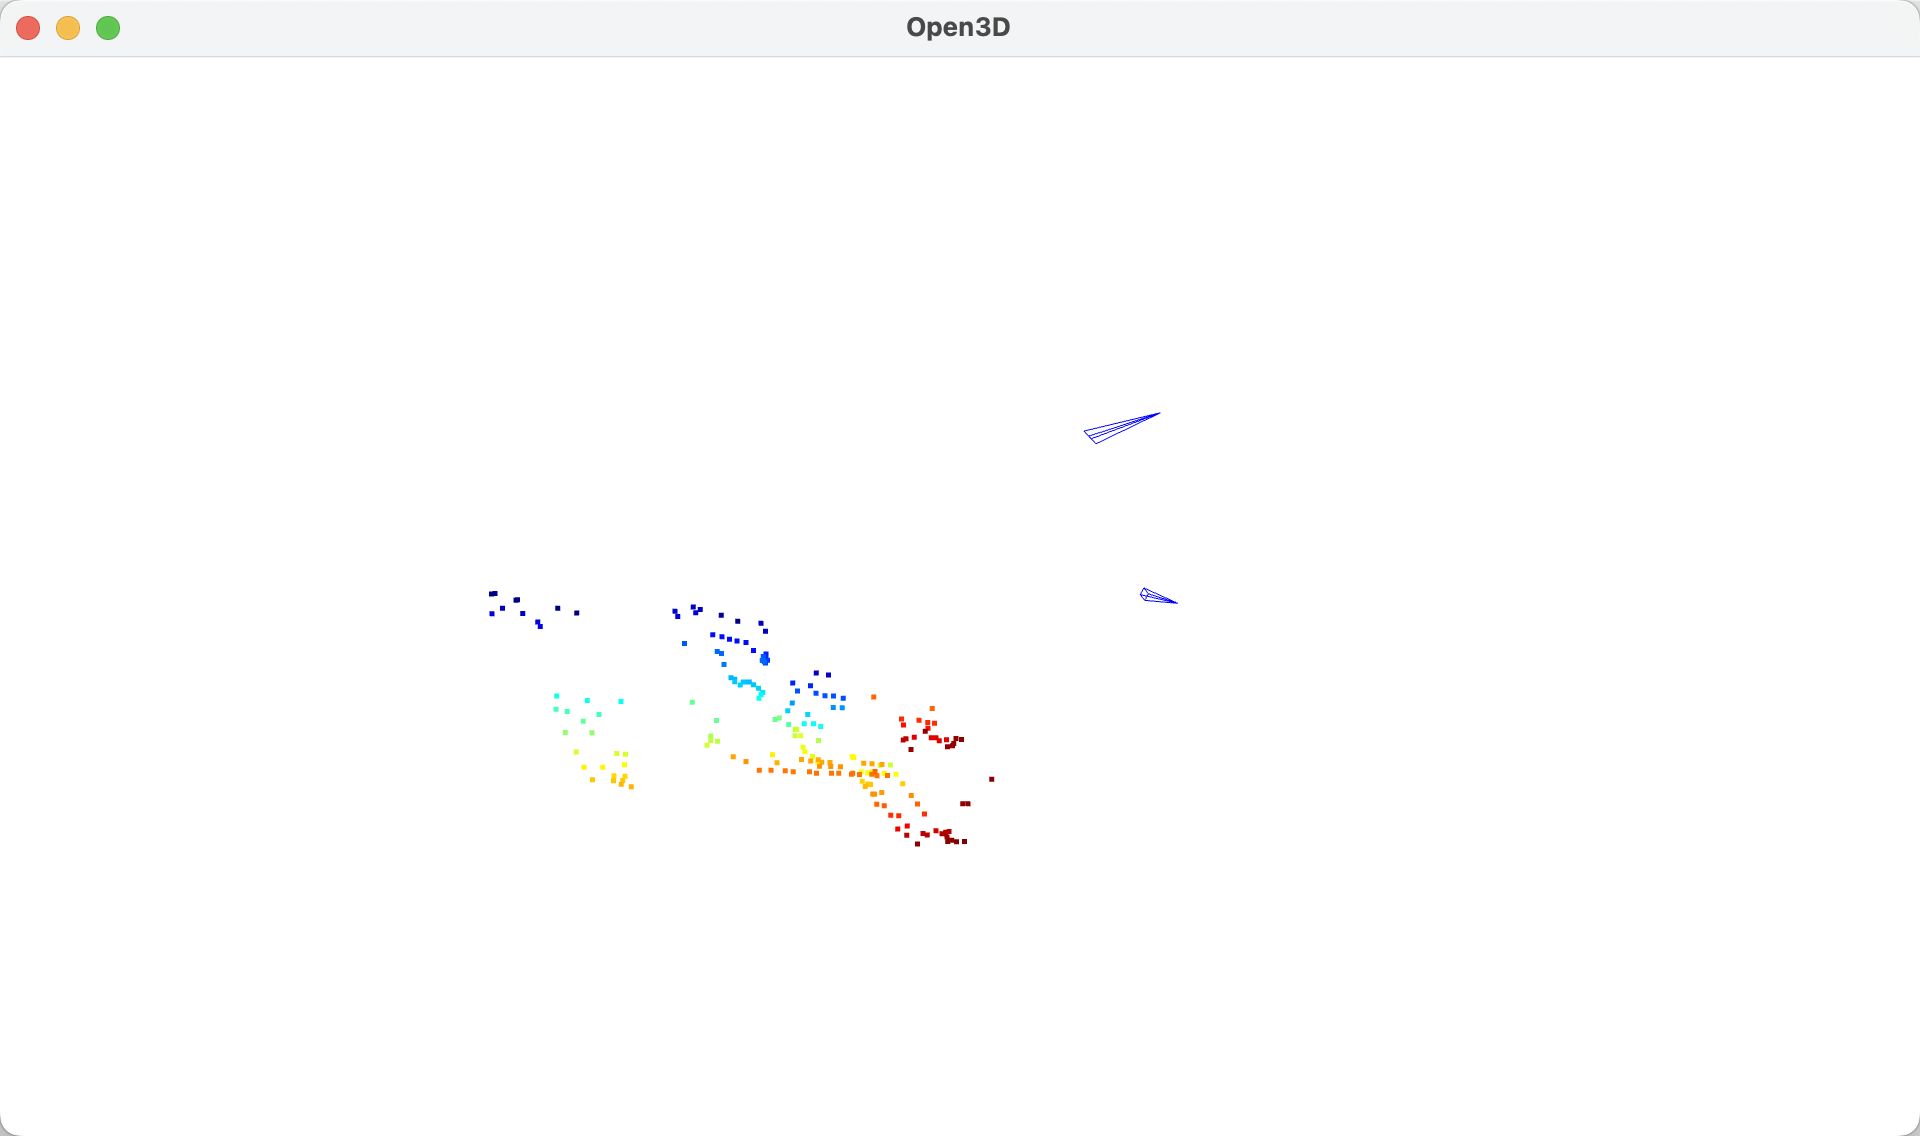
\includegraphics[width=0.3\linewidth]{fig/Q5 right 2.png}
    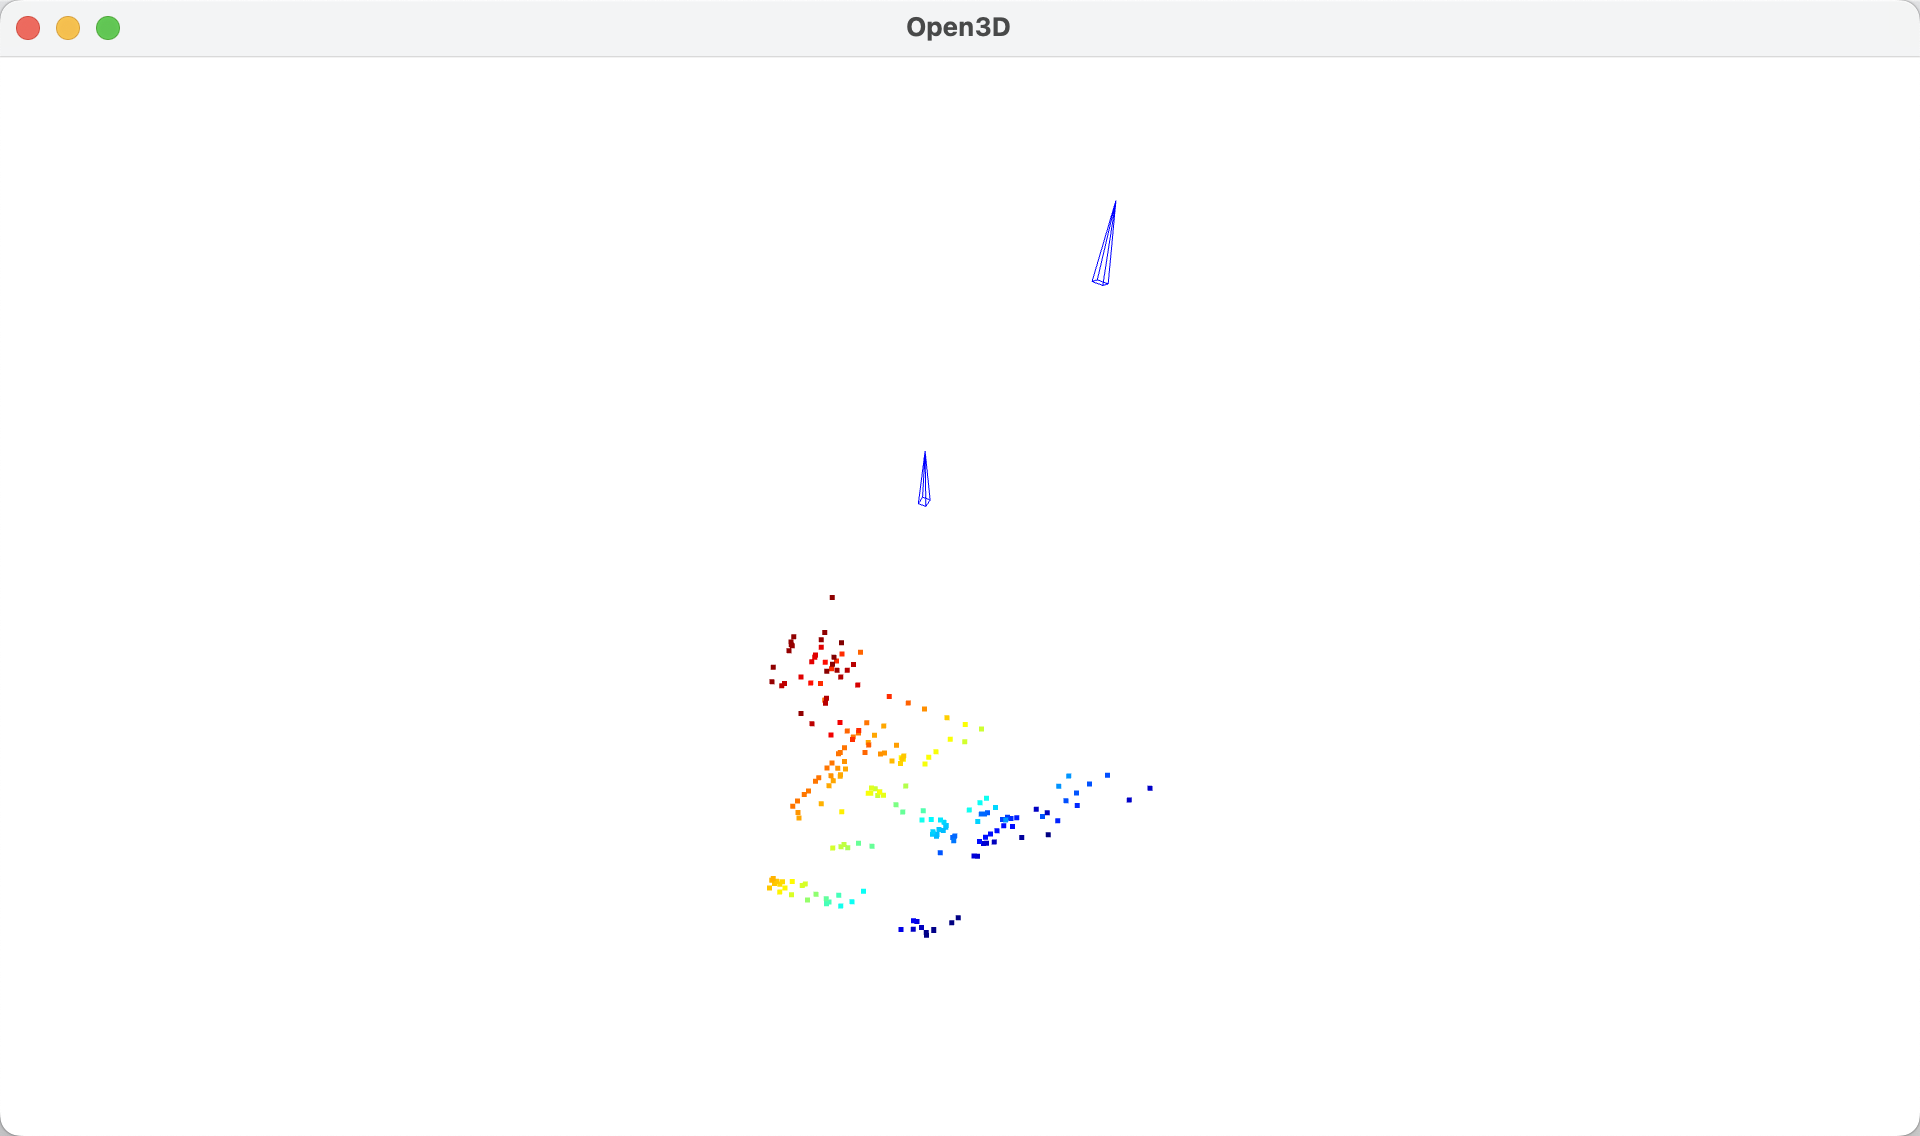
\includegraphics[width=0.3\linewidth]{fig/Q5 right3.png}
\end{center}

\section*{Stereo Estimation}

Now given two camera poses, we could get the relative camera pose and a sparse set of 3D point based on sparse keypoint matching. Could we go further and recover the dense geometry? The answer is yes. In question 6, you will reason a dense point cloud from a pair of images taken at the different views. 

\paragraph{Question 6 (Stereo) [3 pts + 1 bonus pt]:}
Given two images ($\mathbf{I}_1, \mathbf{I}_2$) with ground-truth intrinsic matrices $\mathbf{K}_1, \mathbf{K}_2$, extrinsic matrices $\mathbf{R}_1, \mathbf{t}_1, \mathbf{R}_2, \mathbf{t}_1$. Our goal is to recover a dense correspondence between the two images using stereo matching. 

Computing the dense matching is computationally expensive. We down-sample both images by $s$ times to reduce the computational burden. Could you describe what the updated intrinsic matrices will be? Please report the intrinsics on your write-up and fill in the code to update $\mathbf{K}_1, \mathbf{K}_2$. 

We do notice that the pair of images are not perfectly fronto-parallel. To make matching easier, we will rectify the pair of images such that its epipolar lines are always horizontal. To achieve this, we simply call \texttt{cv2.StereoRectify} function. The updated projection matrices are also returned. Please go through the code and understand what each step does. You do not need to write any code here. 

Finally, we will do stereo matching. Specifically, given a pixel at $(i, j)$ on the left image, we will compute a winner-take-all disparity value that minimizes the sum of square distance (SSD) between a pair of left and right image patches, centered at $(i, j)$ and $(i, j-d)$: 
\[
d[i, j] = \arg\min_d \sum_{m=-w}^{w} \sum_{n=-w}^{w} ( I_1[i+m, j+n] - I_2[i+m, j+n-d] )^2
\]
where $w*2+1$ is the block size and $w$ is an integer. Please do this in a sliding window manner to get the dense disparity map. Please visualize the disparity map you get and include it in your report.

Do you think the disparity you get is satisfactory? You could compare your results against stereo matching results implemented by an off-the-shelf method \texttt{cv2.stereoBM} (we already provide the code). Visualize both methods side-by-side and provide insights into further improving your results. Given disparity map estimation, could you get the dense point cloud? Try to get the point cloud and visualize your point cloud.  (Bonus 1 pt)

\textbf{Answer: } The intrinsic matrix after I scale down by s times is shown as follows, 
\begin{center}
    \small
    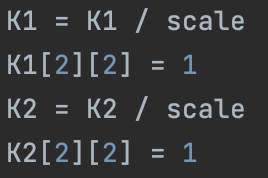
\includegraphics[width=0.2\linewidth]{fig/q6function2.png}
\end{center}
To be specific, the $f_x, f_y, c_x, c_y$ are all divided by $s$ while other parameter remain the same.

Given max disp as 128 and block size as 7, the disparity map and its compare with cv2.stereoBM's output is shown as follows.
\begin{center}
    \small
    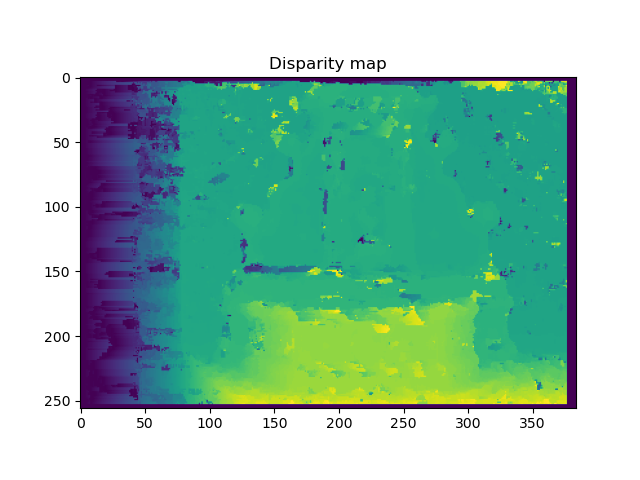
\includegraphics[width=0.35\linewidth]{fig/q6disparity.png}
    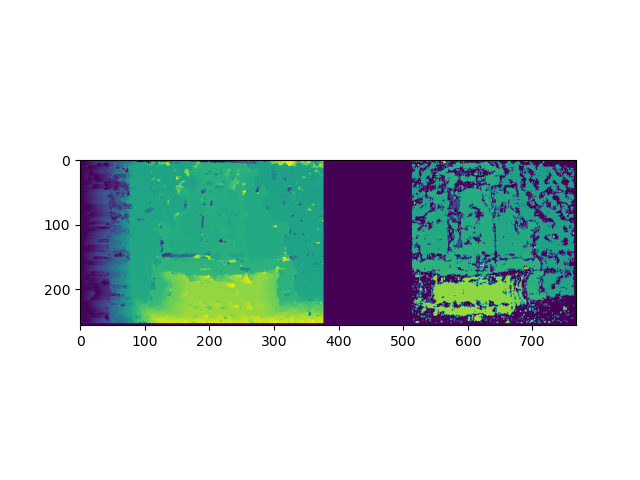
\includegraphics[width=0.35\linewidth]{fig/q6disparitycompare.png}
\end{center}
The sliding window function I use here is shown as follows, I also output and visulize the depth map:
\begin{center}
    \small
    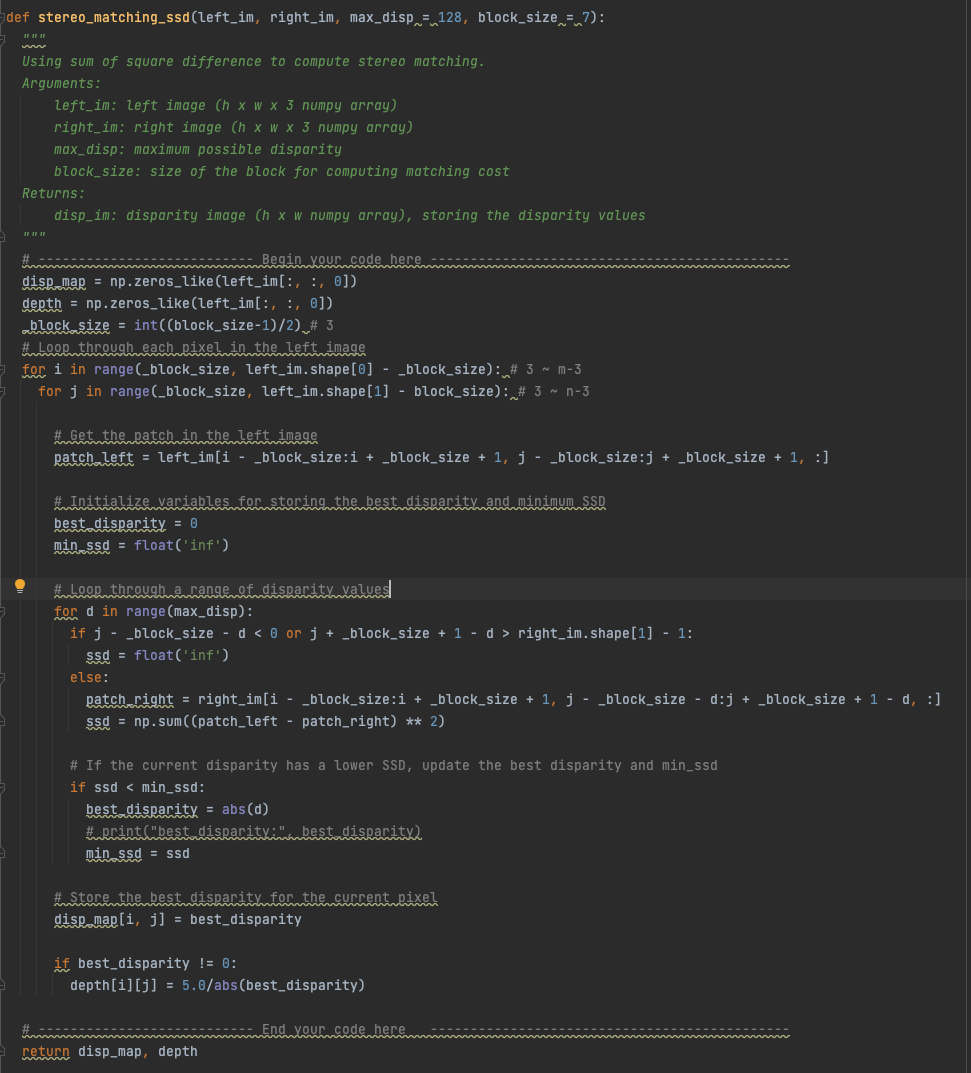
\includegraphics[width=0.35\linewidth]{fig/q6function.png}
\end{center}
The result is clearly not satisfied. There are several ways to improve it. Firstly, if we add the max disp, the algorithm has a larger receptive field, thus it is possible to have a better performance. Secondly, if I increase the sliding window size, the result will be more stable and convincing since it recieves more pixel information in each sliding window. However, the disadvantage of this is that the computing time will increase significantly when we make those two hyperparameter larger. 

The other way to improve performance is using other methods to compute difference between each sliding windows. Besides SSD, I try SAD and normalized correlations here. The function is shown as follows:
\begin{center}
    \small
    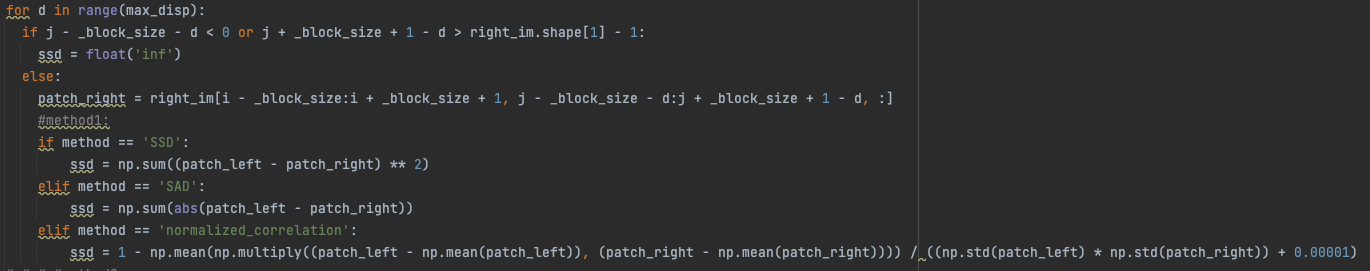
\includegraphics[width=0.35\linewidth]{fig/q6multicalculationfunction.png}
\end{center}
For the SAD, the output is shown as follows, it seems like it has the same performance with SSD, however, it's computing time is smaller. I still use max disp as 128 and block size as 7 here.
\begin{center}
    \small
    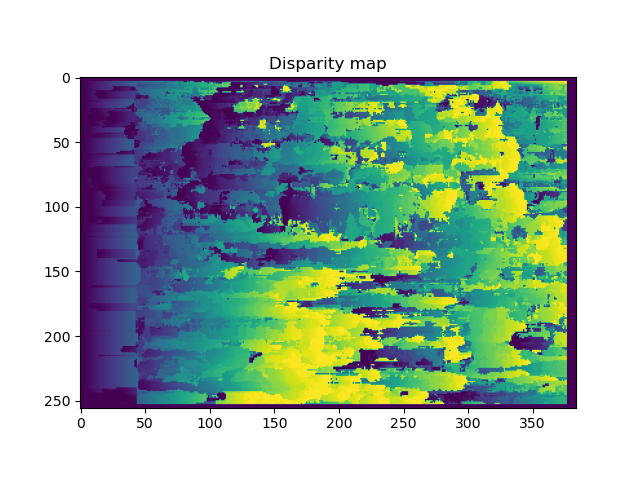
\includegraphics[width=0.35\linewidth]{fig/q6SADoutput.png}
    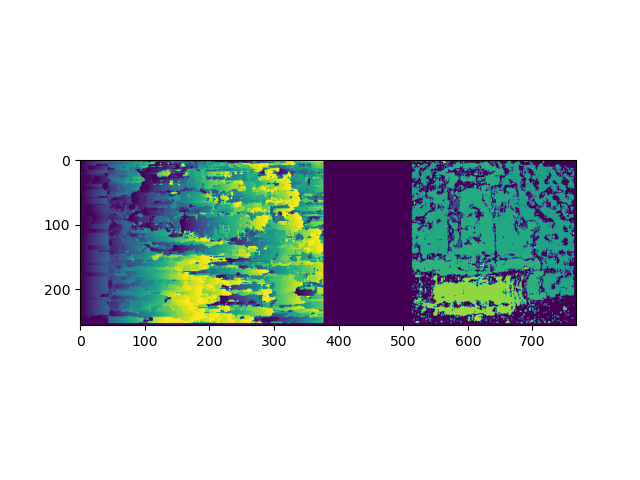
\includegraphics[width=0.35\linewidth]{fig/q6SADcompared.png}
\end{center}
For normalized correlations, the result is shown as follows, it has a little better performance by has better performance in small patterns, however, its computing time is much more larger than the previous two. 
\begin{center}
    \small
    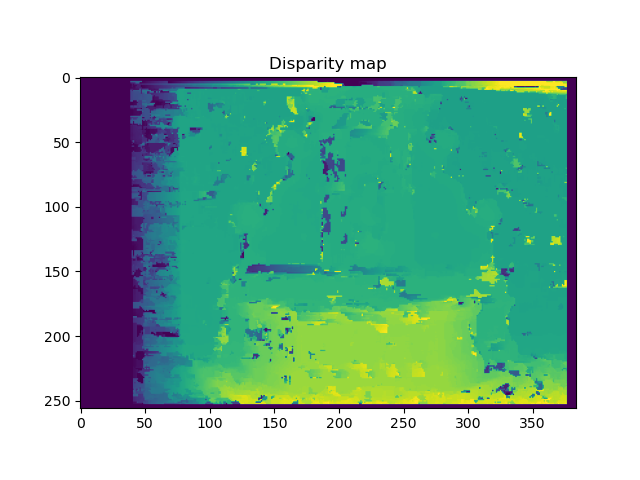
\includegraphics[width=0.35\linewidth]{fig/q6ncoutput.png}
    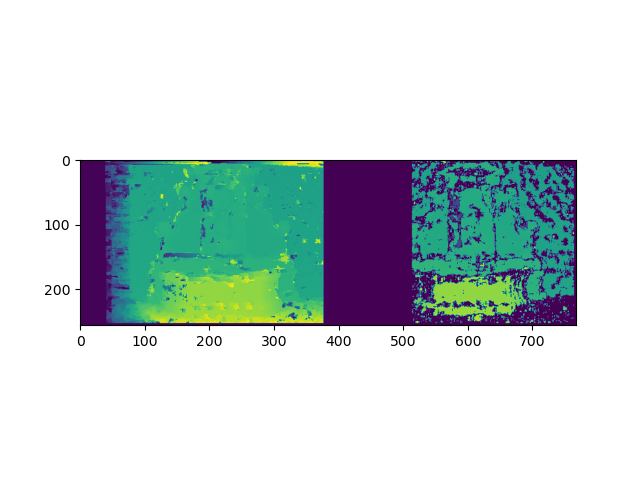
\includegraphics[width=0.35\linewidth]{fig/Q6nccompared.png}
\end{center}
\textbf{Bonus Answer: } In this section, I draw the dense point cloud with following four steps:

1. I got the depth map based on focal length, basline and disparity I got from Q6, since the cameras are rectified, the basline is on x-axis. The equation is shown as follows. There are two ways to calculate distance when disparity reaches 0, the first one is add it with epsilon, which is a very small number while the other way is define depth map as inf when disparity reaches 0.

$depth map = np.where(disparity != 0, (focallength * baseline) / disparity, np.inf)$

2. the second step is adding depth information as z-value to create dense point clouds.

3. the third stpe is converting camera coordinate system to world coordinate system.

4. the last step is create point cloud by o3d.geometry.PointCloud() and adding its points and colors to it.

The output of dense cloud point with first method to calculate depth map is shown as follows, the epsilon of left image is set as 0.001 while the right image's epsilon is 0.1:
\begin{center}
    \small
    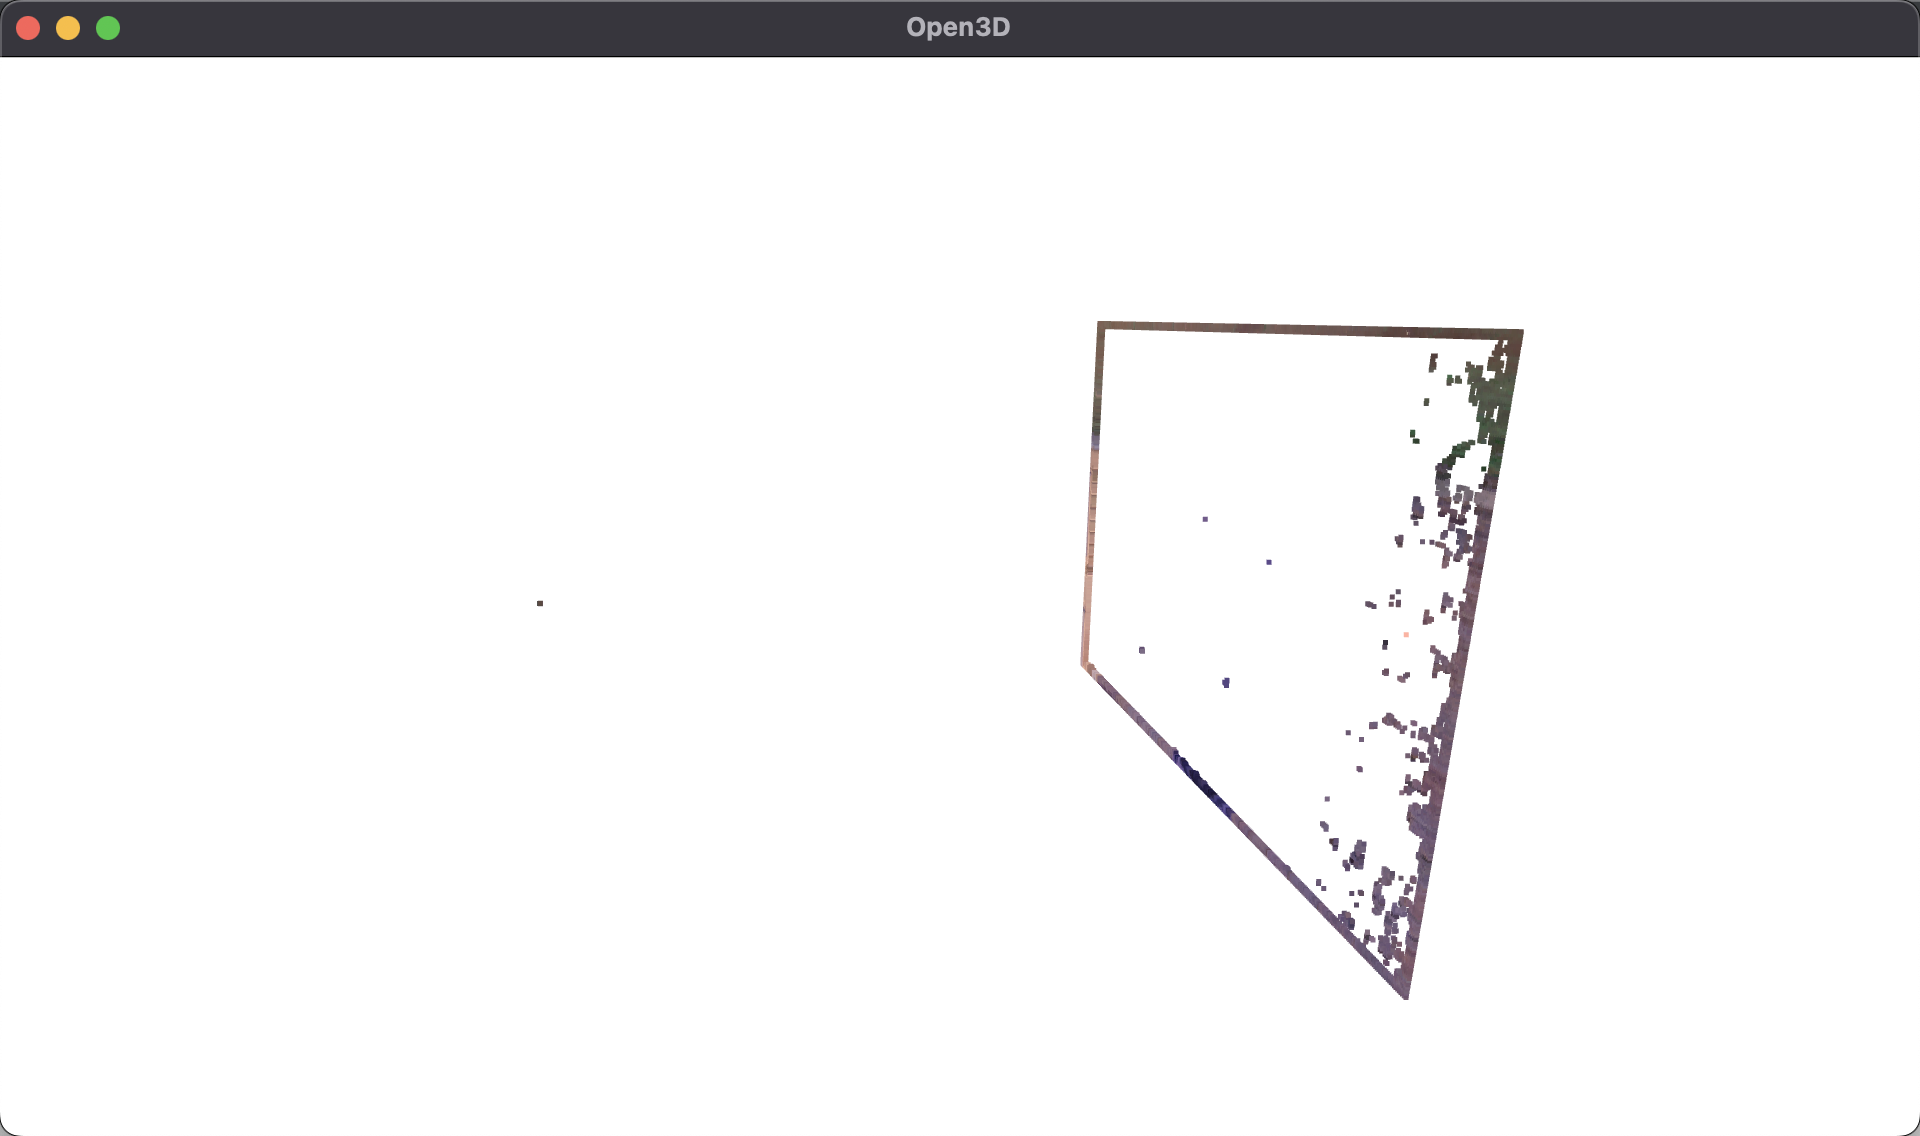
\includegraphics[width=0.35\linewidth]{fig/q6bonus0.001.png}
    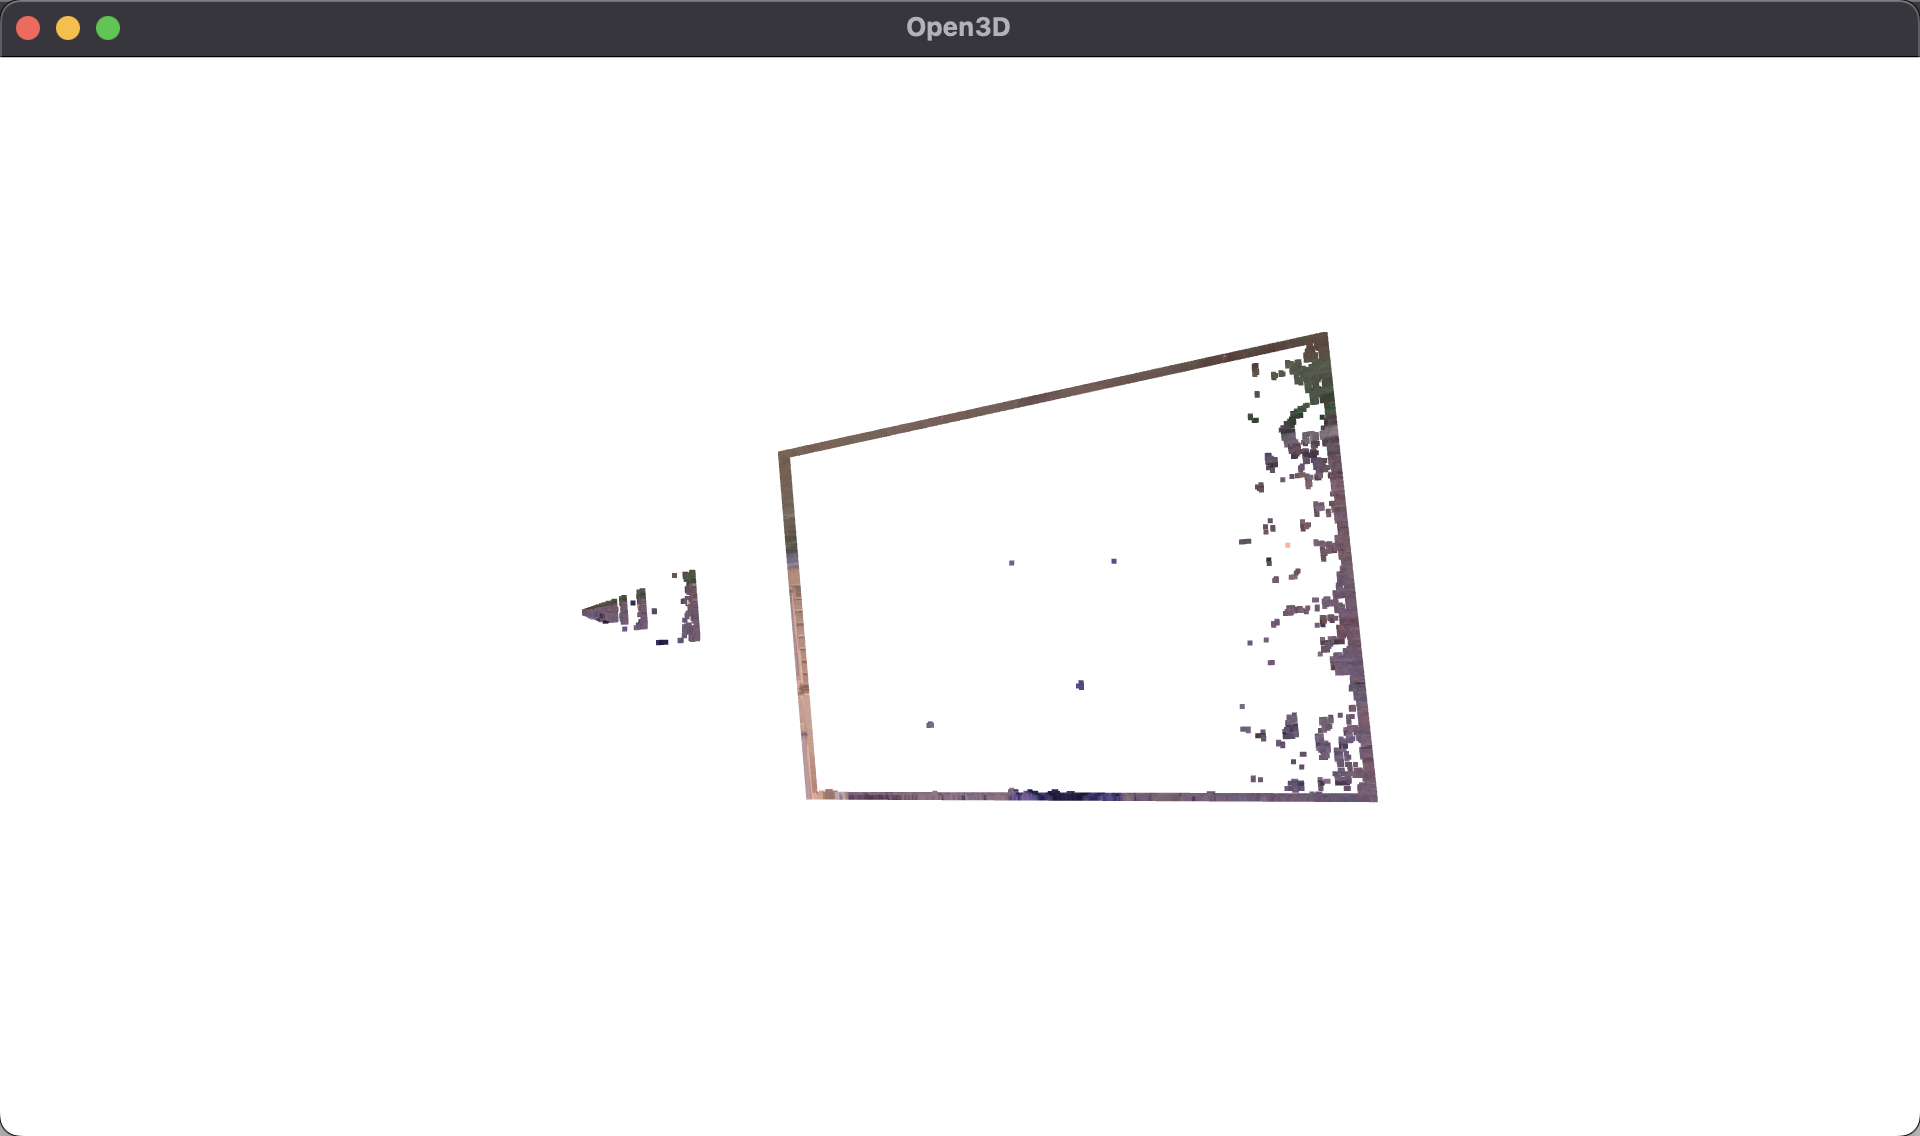
\includegraphics[width=0.35\linewidth]{fig/Q6bonus0.1.png}
\end{center}
The output of dense cloud point with second method to calculate depth map is shown as follows, I show it with three dufferent viewing perspectives.
\begin{center}
    \small
    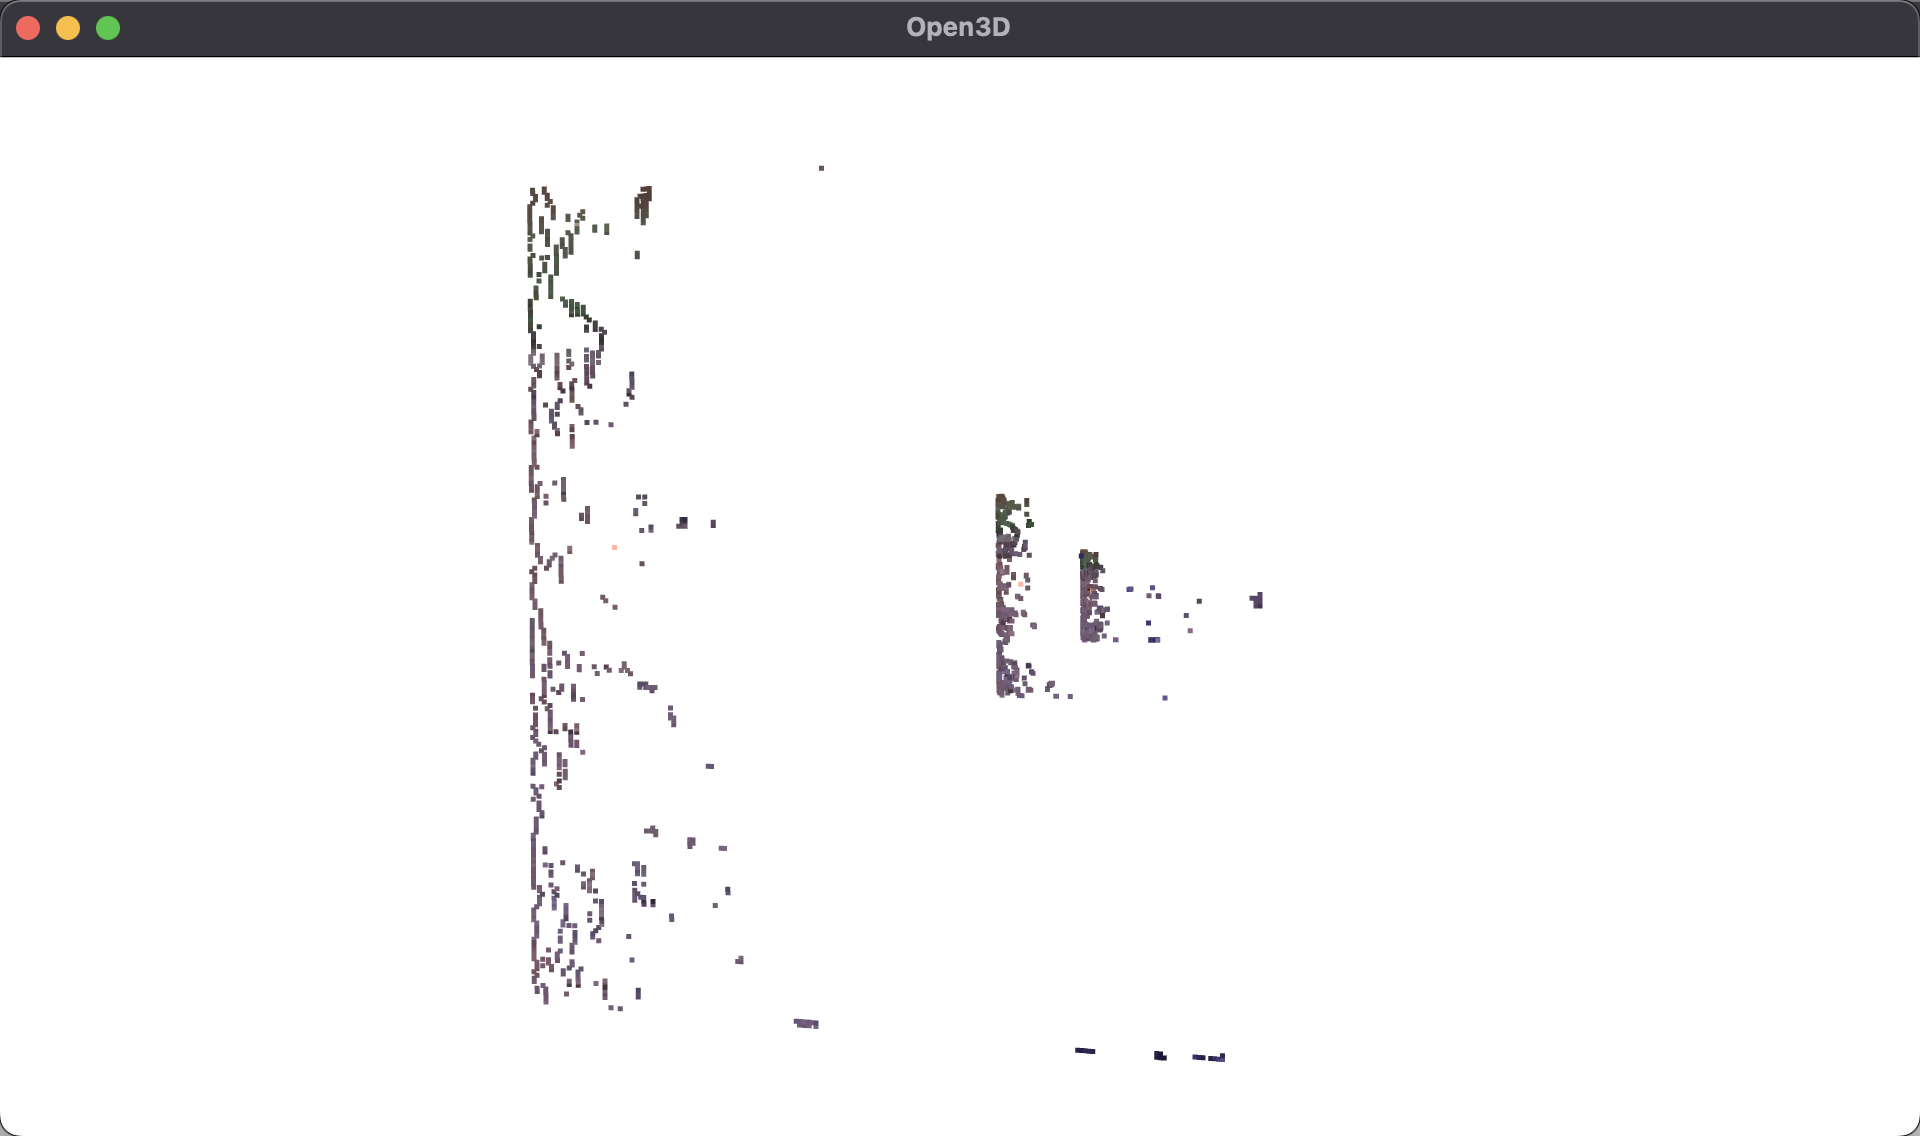
\includegraphics[width=0.35\linewidth]{fig/Q6bouns1.png}
    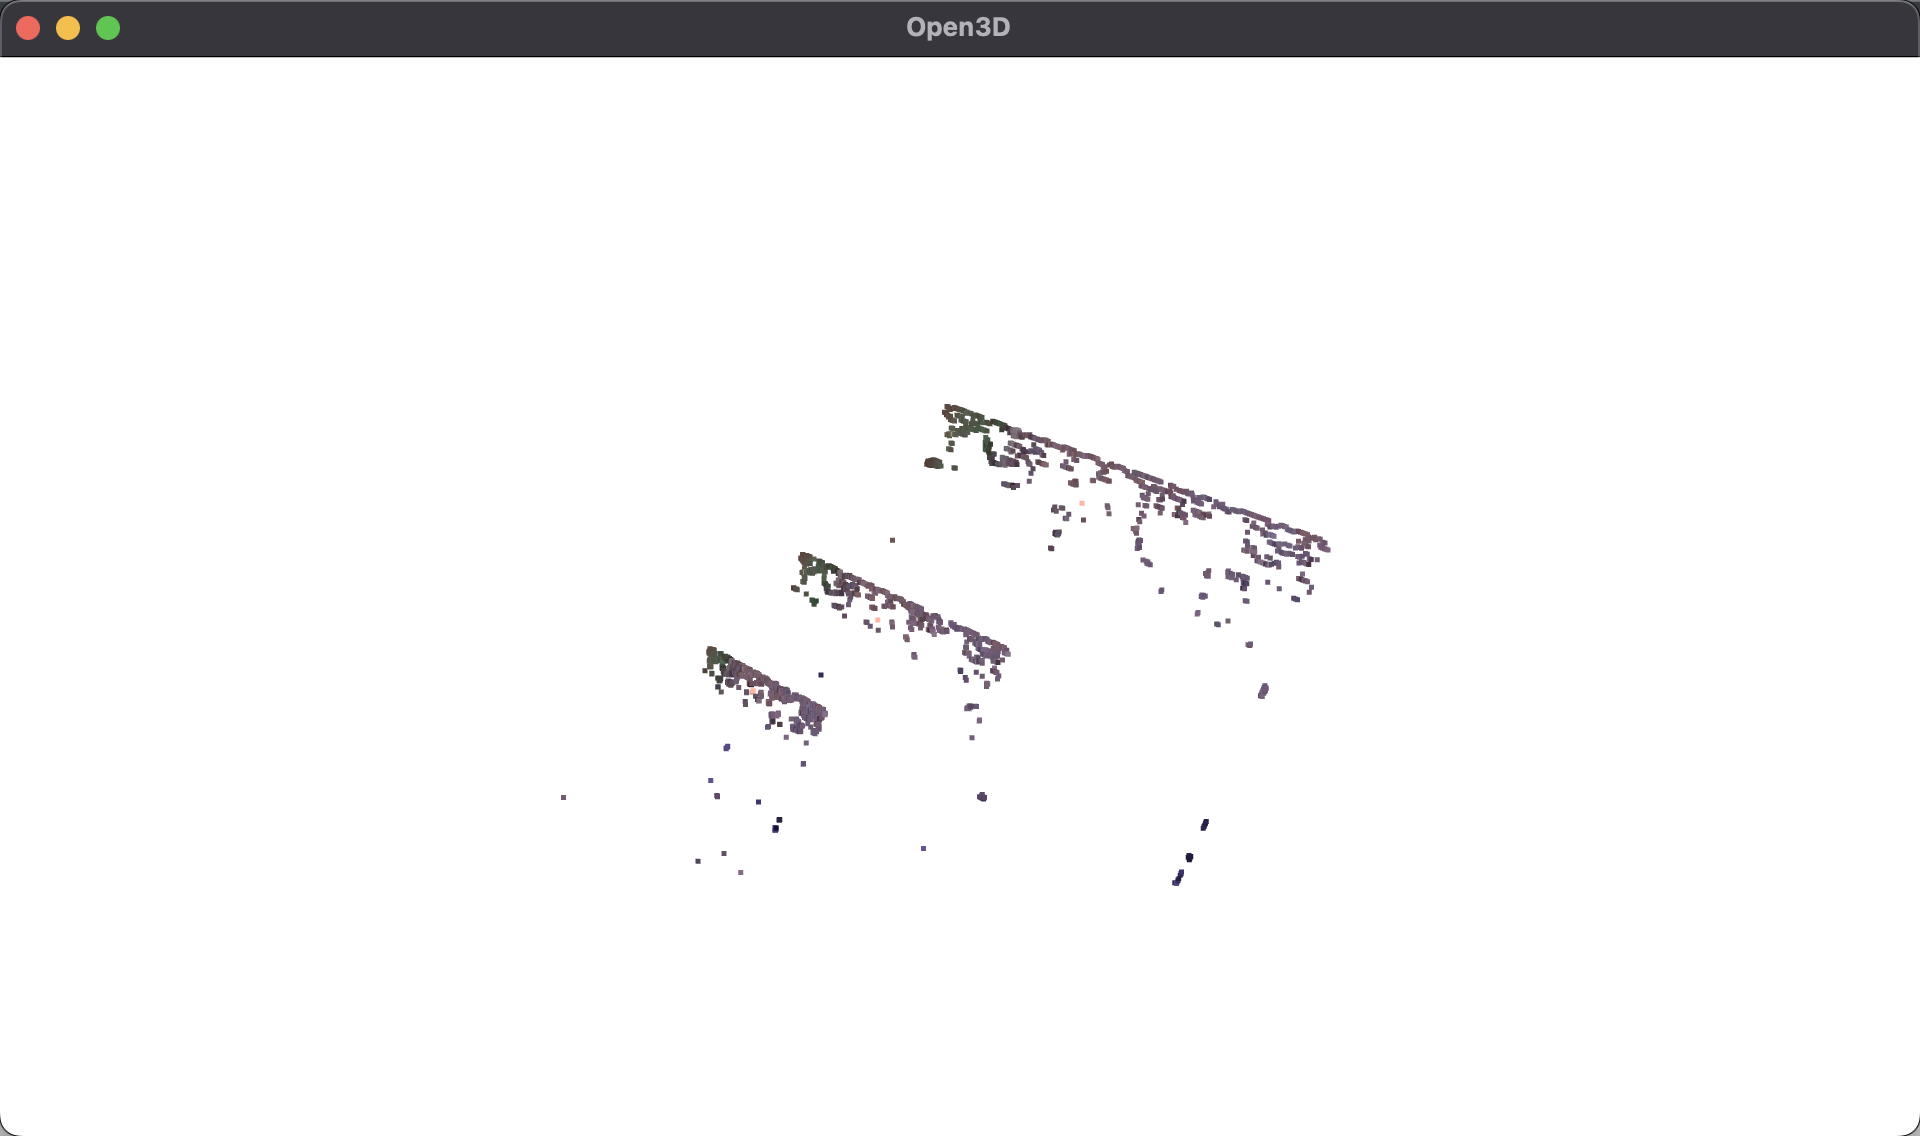
\includegraphics[width=0.35\linewidth]{fig/Q6bonus2.png}
    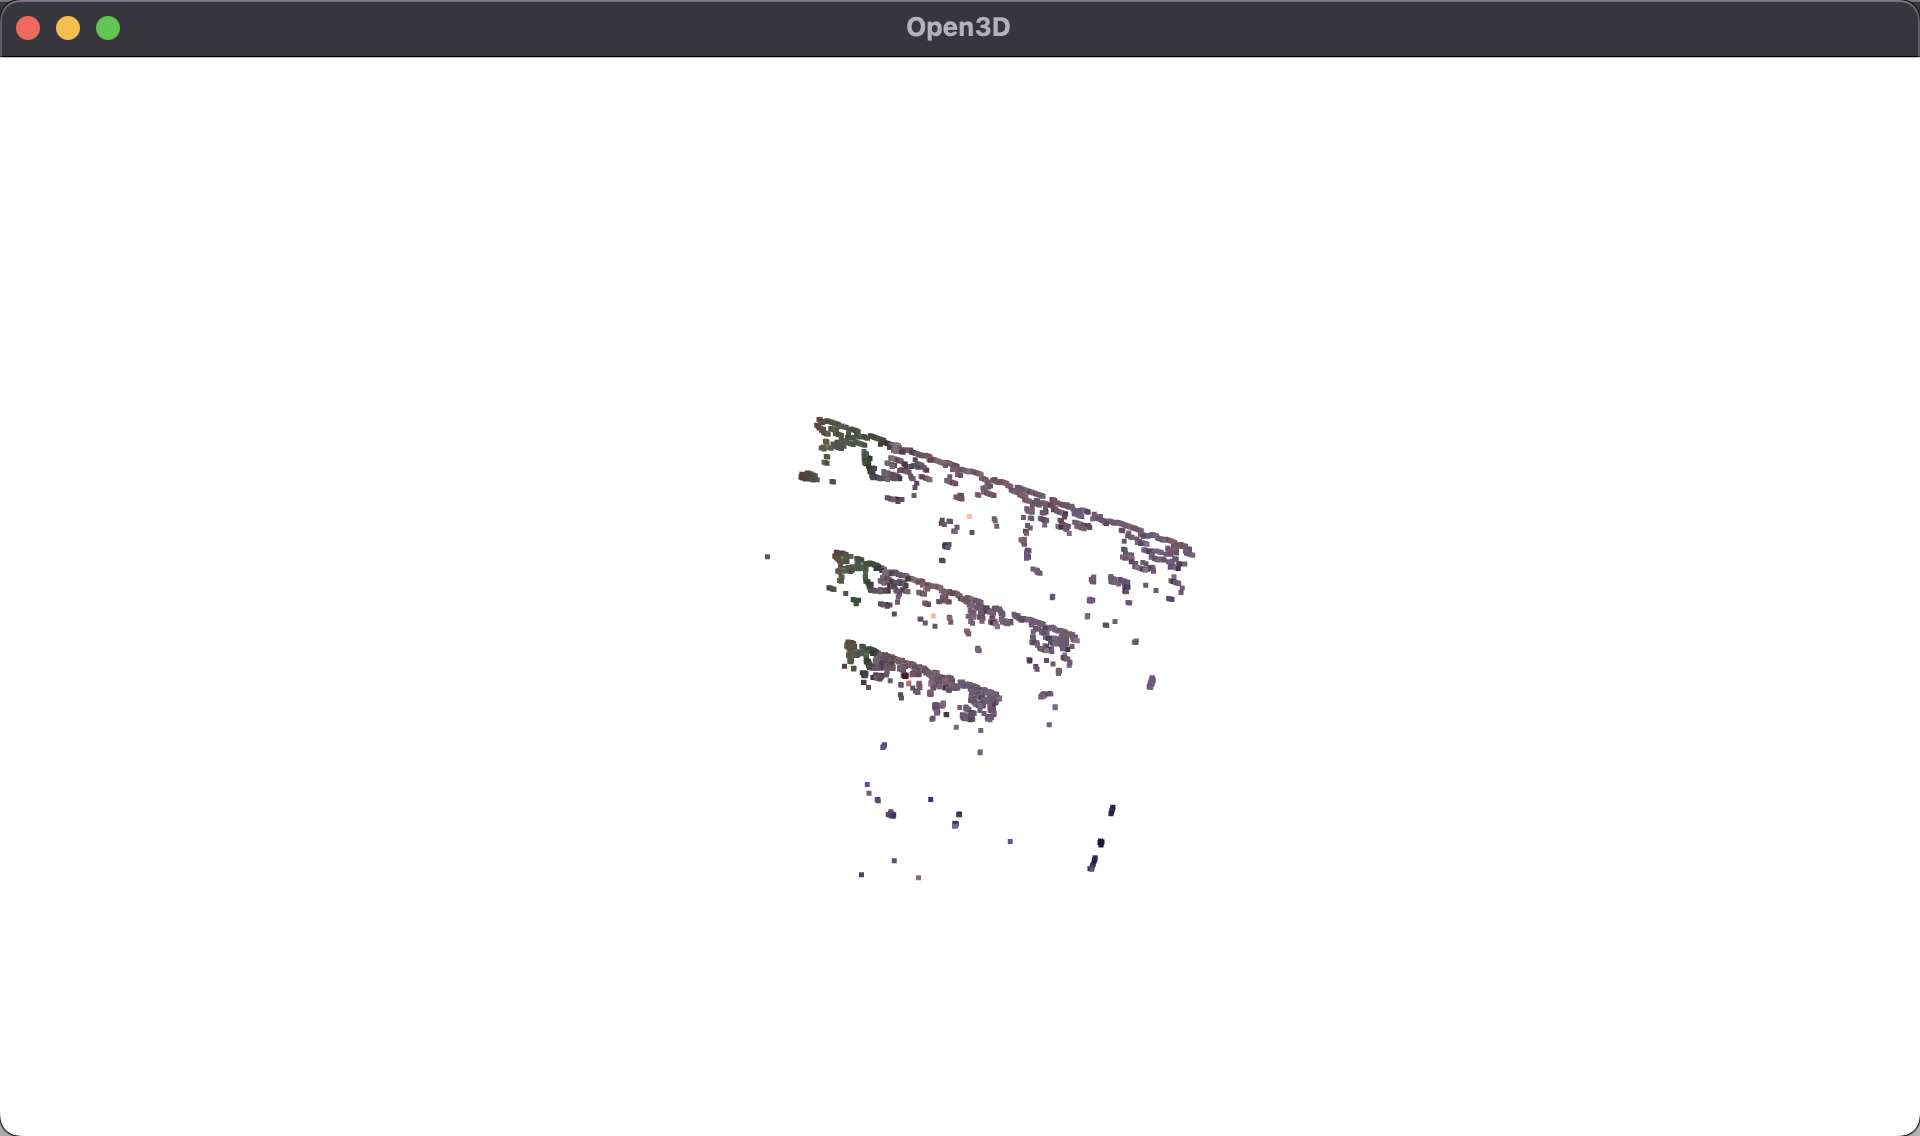
\includegraphics[width=0.35\linewidth]{fig/Q6bonus3inf.png}
\end{center}


% \section*{Bundle Adjustment} 

% \paragraph{Question 6 (Jacobian Calculation) [pt]:}
% # For this question, please use our provided notation, and derive the Jacobian matrix with respect to 3d point $X^i$. We denote the rotation matrix as $R_a$, translation for camera i as $t_a$, intrinsic matrix  as $K_a$ for camera pose a. $x_a^i$ represent the 2d point corresponds to the 3d point $X^i$ in camera pose $a$. In your solution, make sure to give details about how you derive the Jacobian of E with respect to $X_i$.
% \begin{equation*}
%     \begin{split}
%         \underset{X, R, t}{\text{min}} ~E = \underset{i}{\sum} \Vert K_a[R_a | t_a] X^i - x^i_a\Vert
%     \end{split}
% \end{equation*}
% \paragraph{Question 7 (Gaussian Newton Update)~ [pt]:} 
% For this question, please implement your estimated Jacobian for a single 3d point, and implement Gaussian Newton Update step. You are given the initial estimated for 3d point $X^i$, together with ground-truth camera poses $R$, $t$, and camera intrinsics $K$. For simplicity, the bundle adjustment for this problem only optimizes 3d points location $X$. Please report the residual error in your PDF report.

\paragraph{Question 7 (Structure-from-Motion) [bonus 3 pts]:}
We believe you have a thorough understanding of multi-view geometry now. This bonus question will expand the two-view structure-from-motion and stereo estimation problem into multiple views. You have two directions to win the three bonus points: 1) Write your own mini bundle adjustment solver and run it on the fountain dataset. You could leverage Ceres, g2o, GTSAM libraries as your non-linear least square solver, but you need to derive the Jacobian of the energy terms and write your own code to initialize camera poses and 3D points, based on two-view geometry; 2) Collect your own data and utilize Colmap (https://demuc.de/colmap/) to run the full MVS pipeline. This includes correspondences matching, initialization, bundle adjustment, multi-view stereo matching, and depth fusion. Visualize your camera trajectories, sparse point cloud from SFM, and the final dense point cloud from multi-view stereo. Try your best to get the most creative and visually appealing results. We will choose the top solutions in each direction and announce them in the class. 
\end{document}. 

\grid
\grid